\section{Event Categorization}\label{section:higgs_categorization}
For the purpose of increasing the sensitivity of the analysis, the next step performed is the categorization of events into different subclasses. The basic idea is to utilize the knowledge about two important characteristics of the search needs: the physics of interest, differences between the production processes, and the fact that muon detectors intrinsically have better resolution for certain geometrical regions (barrel vs endcap). Using this information will allow to substantially increase the significance of the Standard Model signal over the expected background.

\subsection{Baseline Categorization}
During the CMS Run I analysis campaign \cite{CMSHiggsRunI}, the categorization procedure used was optimized to separate VBF like events from the rest by requiring the presence of at least 2 jets, pssing the Jet Selections, and going into the opposite ends of the detector and employing large Missing Transverse Energy (MET) selection. Moreover, the resolution of Muon System is significantly better in the Barrel region than in the Endcap, therefore the space is subdivided in $\eta$ variable by defining:
\begin{itemize}
  \item Barrel: $|\eta| < 0.8$
  \item Overlap: $|\eta| \ge 0.8$ \& $|\eta| < 1.6$
  \item Endcap: $|\eta| \ge 1.6$ \& $|\eta| < 2.1$
\end{itemize}
Furthermore, once a Higgs candidate pair is constructed, each muon is tagged according to the region of the detector it was reconstructed in. The exact selections applied in the baseline categorization procedure are:
\begin{itemize}
  \item $njets \ge 2$ \& $p_{t}^{j1} > 40$ GeV \& $p_{t}^{MET} < 40$ GeV - require at least 2 jets with thresholds on p$_t$ of the leading jet and Missing Energy Transverse.
    \begin{itemize}
      \item ''VBFTight'' Category: $m_{jj} > 650$ GeV \& $|\Delta \eta| > 3.5$ - category targeting the Vector Boson Fusion production mechanism. The signature is the presence of 2 jets with a large invariant mass and going into opposite ends of CMS.
      \item ''GFTight'' Category: if not VBFTight \& $m_{jj} > 250$ GeV \& $p_{t}^{\mu\mu} > 50$ GeV. In this category, we target Gluon Fusion production together with what does not pass the VBF-like selections.
      \item ''GFLoose'' Category: here collect everything that does not pass the VBFTight and GFTight selections.
    \end{itemize}
  \item $njets \le 1$ - the biggest portion of the events will have only 1 or 0 jets total per event (that pass previously discussed selections).
    \begin{itemize}
      \item ''01JetsTight'' Category - $p_t^{\mu\mu} \ge 25$ GeV. The only discriminating variable we are left with at this point is the \pt of the dimuon system that typically has higher values for the signal events.
        \begin{itemize}
          \item ''01JetsTightBB'': $\mu_{1,2}$ are Barrel
          \item ''01JetsTightBE'': $\mu_{1}$ is Barrel \& $\mu_2$ is Endcap
          \item ''01JetsTightBO'': $\mu_{1}$ is Barrel \& $\mu_2$ is Overlap
          \item ''01JetsTightEE'': $\mu_{1}$ is Endcap \& $\mu_2$ is Endcap
          \item ''01JetsTightEO'': $\mu_{1}$ is Endcap \& $\mu_2$ is Overlap
          \item ''01JetsTightOO'': $\mu_{1}$ is Overlap \& $\mu_2$ is Overlap
        \end{itemize}
      \item ''01JetsLoose'' Category - Left over events fall into this category.
        \begin{itemize}
          \item ''01JetsLooseBB'': $\mu_{1,2}$ are Barrel
          \item ''01JetsLooseBE'': $\mu_{1}$ is Barrel \& $\mu_2$ is Endcap
          \item ''01JetsLooseBO'': $\mu_{1}$ is Barrel \& $\mu_2$ is Overlap
          \item ''01JetsLooseEE'': $\mu_{1}$ is Endcap \& $\mu_2$ is Endcap
          \item ''01JetsLooseEO'': $\mu_{1}$ is Endcap \& $\mu_2$ is Overlap
          \item ''01JetsLooseOO'': $\mu_{1}$ is Overlap \& $\mu_2$ is Overlap
        \end{itemize}
    \end{itemize}
\end{itemize}

Figures~\ref{fig:higgs_categorization_2jetsall}-~\ref{fig:higgs_categorization_01jetslooseeeeooo} show dimuon mass distributions for all of the terminal categories. For the final analysis, given that both Muon Corrections are producing similar results, Rochester Corrections are used. Data in all of the categories is modeled well by the included backgrounds.
\begin{figure}[htbp]
  \centering
  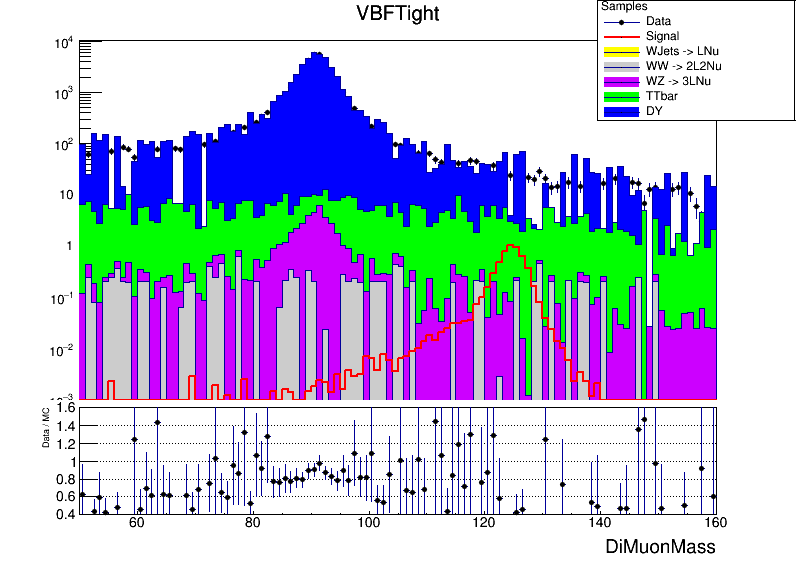
\includegraphics[width=0.65\linewidth]{figures/ch_higgs/distributions/baseline_kalman/distribution__VBFTight__DiMuonMass__logY.png}\\
  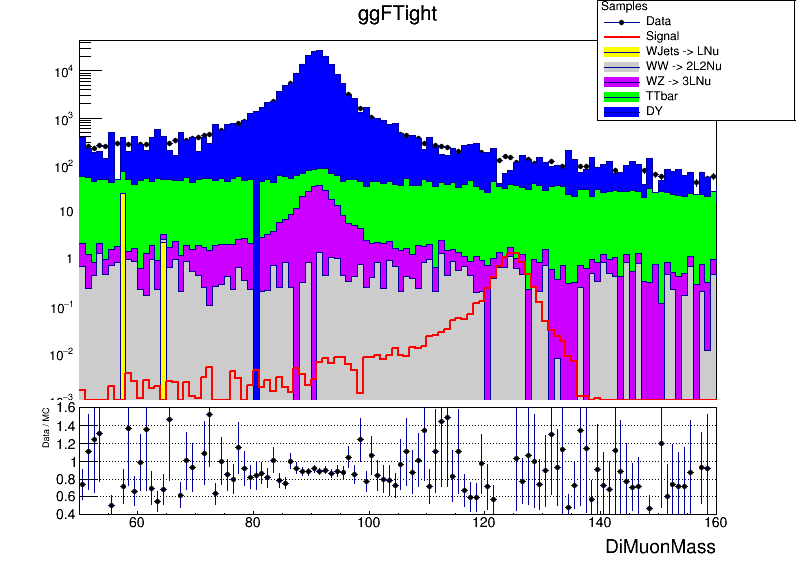
\includegraphics[width=0.65\linewidth]{figures/ch_higgs/distributions/baseline_kalman/distribution__ggFTight__DiMuonMass__logY.png}\\
  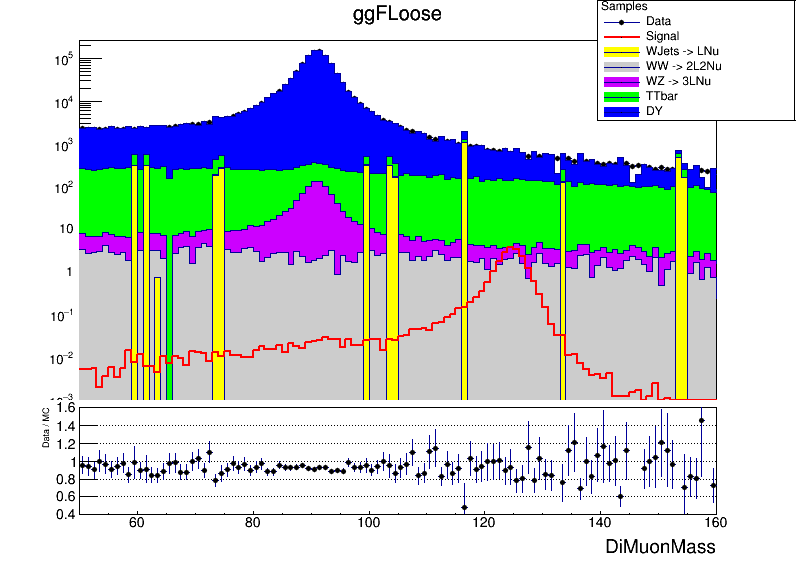
\includegraphics[width=0.65\linewidth]{figures/ch_higgs/distributions/baseline_kalman/distribution__ggFLoose__DiMuonMass__logY.png}
  \caption{Mass Distributions VBFTight (Top), GFTight (Middle) and GFLoose (Bottom) Categories.}
  \label{fig:higgs_categorization_2jetsall}
\end{figure}
\begin{figure}[htbp]
  \centering
  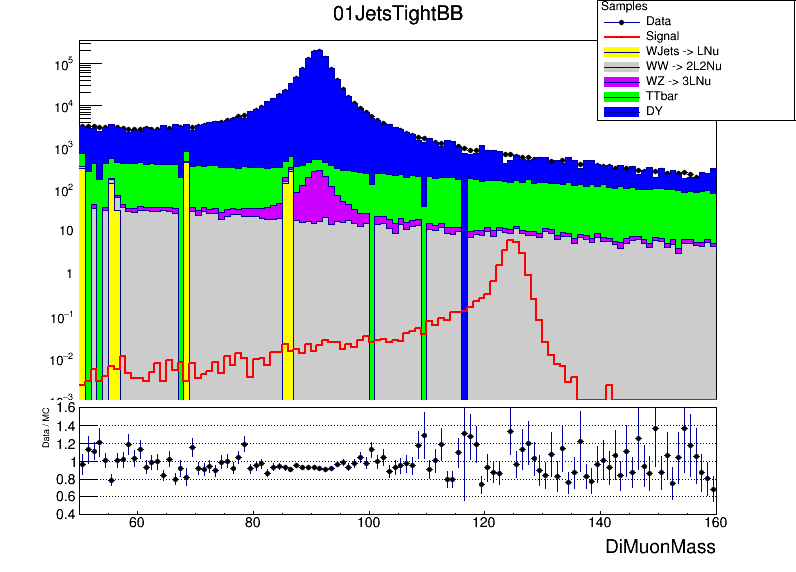
\includegraphics[width=0.65\linewidth]{figures/ch_higgs/distributions/baseline_kalman/distribution__01JetsTightBB__DiMuonMass__logY.png}\\
  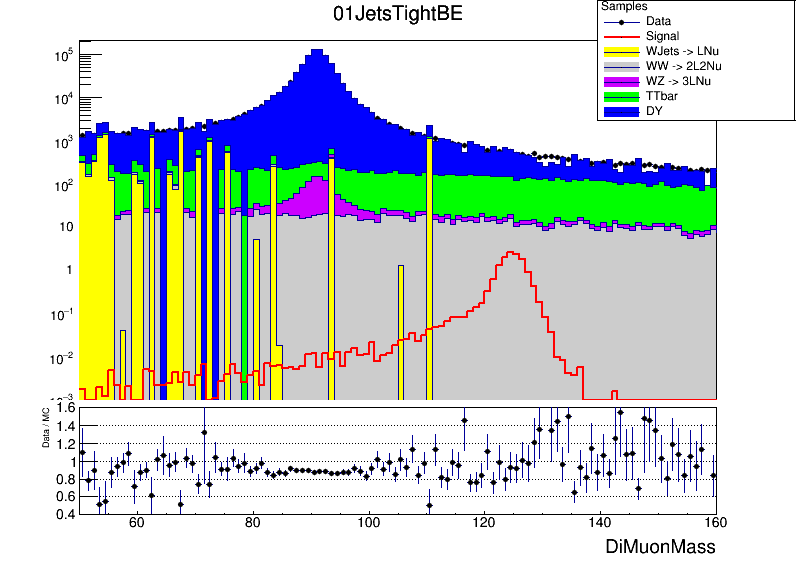
\includegraphics[width=0.65\linewidth]{figures/ch_higgs/distributions/baseline_kalman/distribution__01JetsTightBE__DiMuonMass__logY.png}\\
  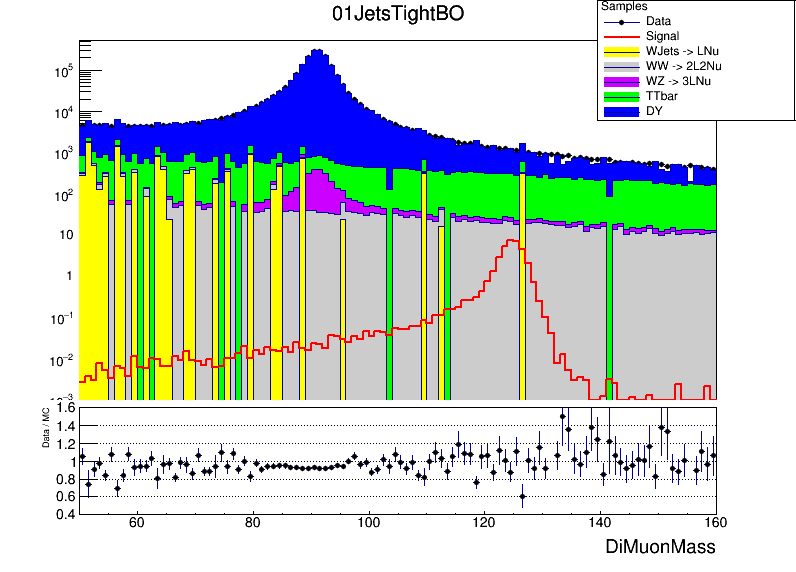
\includegraphics[width=0.65\linewidth]{figures/ch_higgs/distributions/baseline_kalman/distribution__01JetsTightBO__DiMuonMass__logY.png}
  \caption{Mass Distributions 01JetsTightBB (Top), 01JetsTightBE (Middle) and 01JetsTightBO (Bottom) Categories.}
  \label{fig:higgs_categorization_01jetstightbbbebo}
\end{figure}
\begin{figure}[htbp]
  \centering
  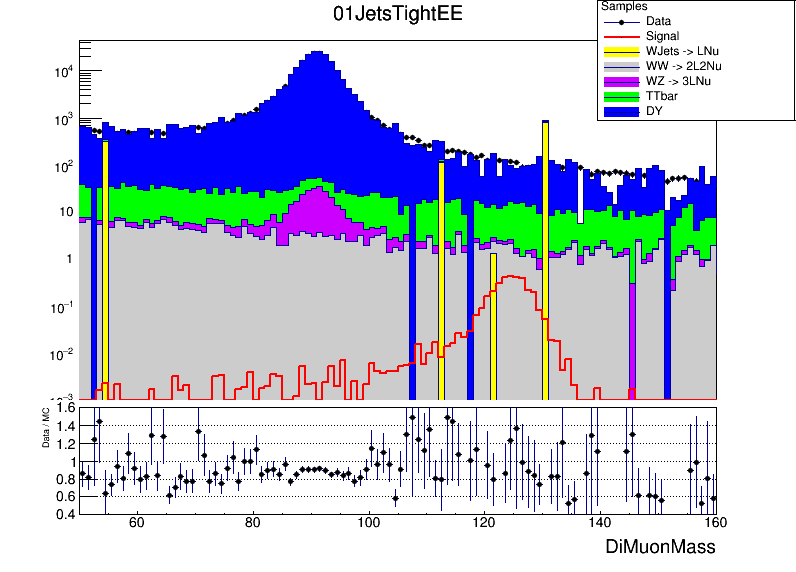
\includegraphics[width=0.65\linewidth]{figures/ch_higgs/distributions/baseline_kalman/distribution__01JetsTightEE__DiMuonMass__logY.png}\\
  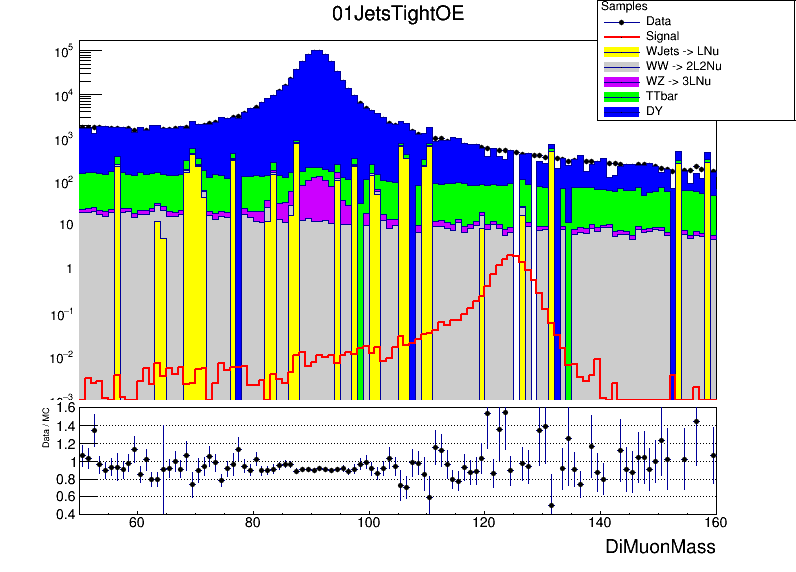
\includegraphics[width=0.65\linewidth]{figures/ch_higgs/distributions/baseline_kalman/distribution__01JetsTightOE__DiMuonMass__logY.png}\\
  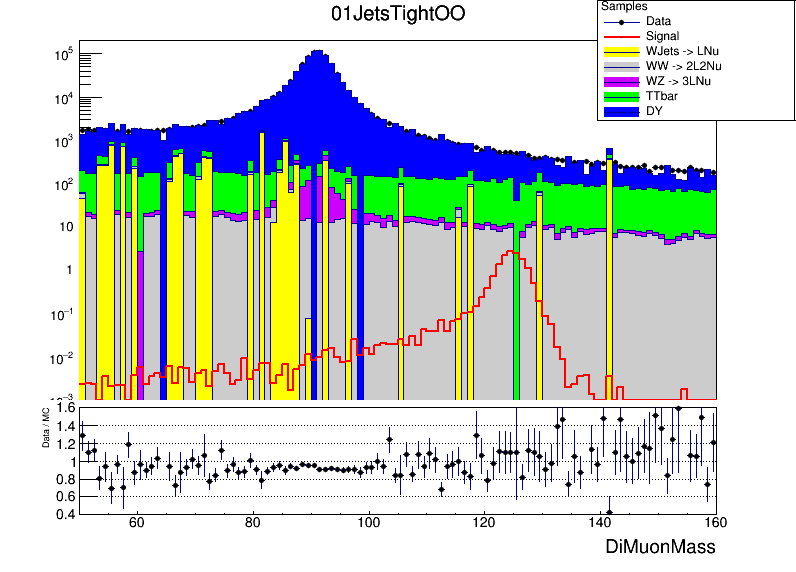
\includegraphics[width=0.65\linewidth]{figures/ch_higgs/distributions/baseline_kalman/distribution__01JetsTightOO__DiMuonMass__logY.png}
  \caption{Mass Distributions 01JetsTightEE (Top), 01JetsTightOE (Middle) and 01JetsTightOO (Bottom) Categories.}
  \label{fig:higgs_categorization_01jetstighteeeooo}
\end{figure}
\begin{figure}[htbp]
  \centering
  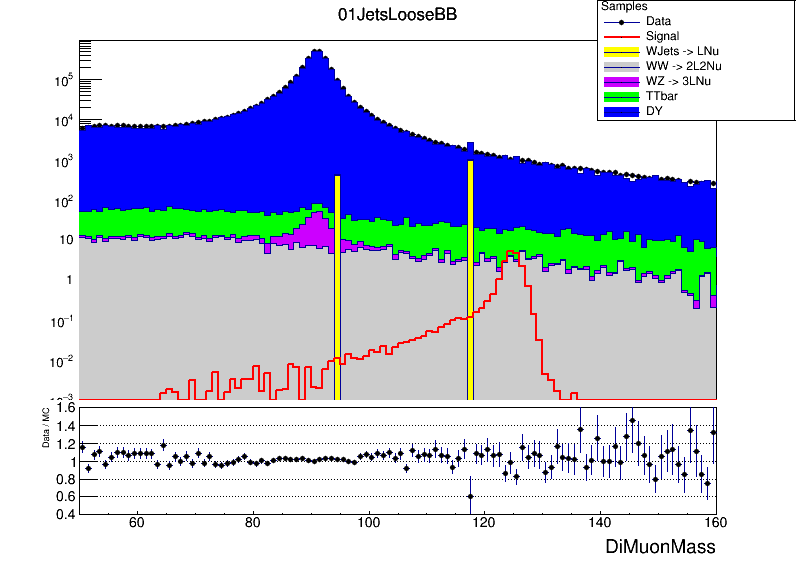
\includegraphics[width=0.65\linewidth]{figures/ch_higgs/distributions/baseline_kalman/distribution__01JetsLooseBB__DiMuonMass__logY.png}\\
  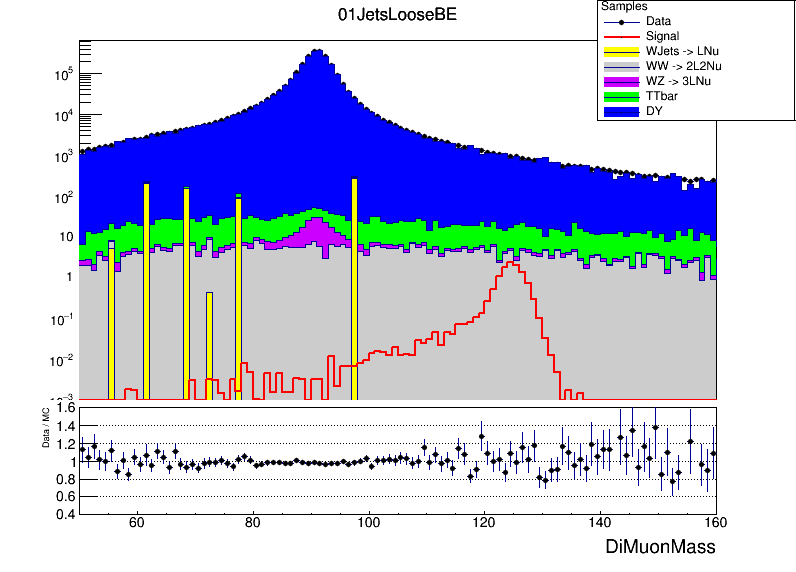
\includegraphics[width=0.65\linewidth]{figures/ch_higgs/distributions/baseline_kalman/distribution__01JetsLooseBE__DiMuonMass__logY.png}\\
  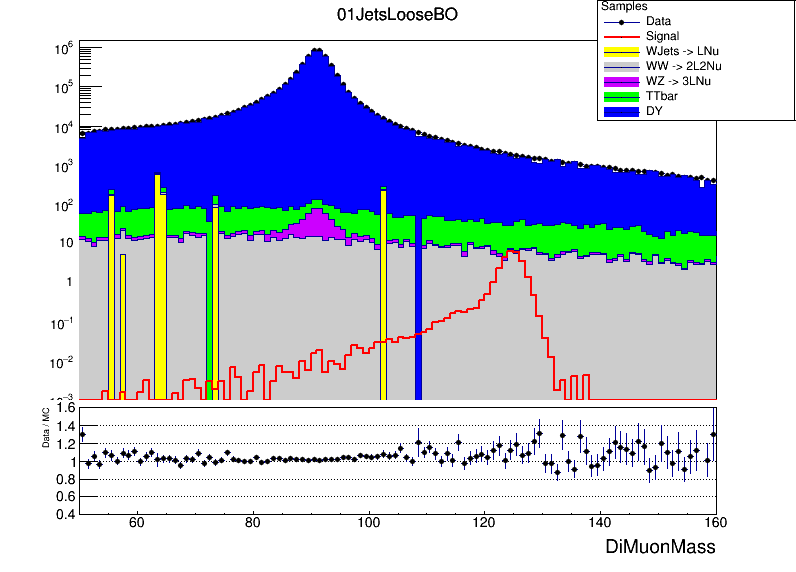
\includegraphics[width=0.65\linewidth]{figures/ch_higgs/distributions/baseline_kalman/distribution__01JetsLooseBO__DiMuonMass__logY.png}
  \caption{Mass Distributions 01JetsLooseBB (Top), 01JetsLooseBE (Middle) and 01JetsLooseBO (Bottom) Categories.}
  \label{fig:higgs_categorization_01jetsloosebbbebo}
\end{figure}
\begin{figure}[htbp]
  \centering
  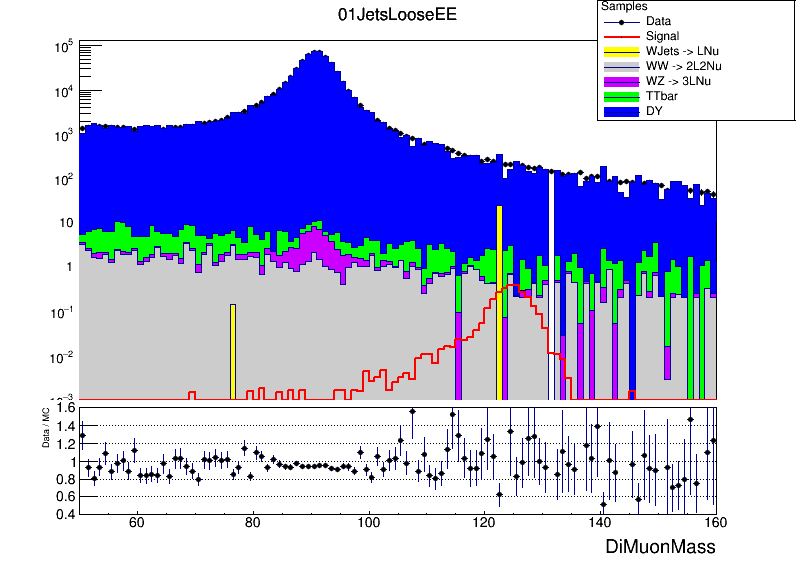
\includegraphics[width=0.65\linewidth]{figures/ch_higgs/distributions/baseline_kalman/distribution__01JetsLooseEE__DiMuonMass__logY.png}\\
  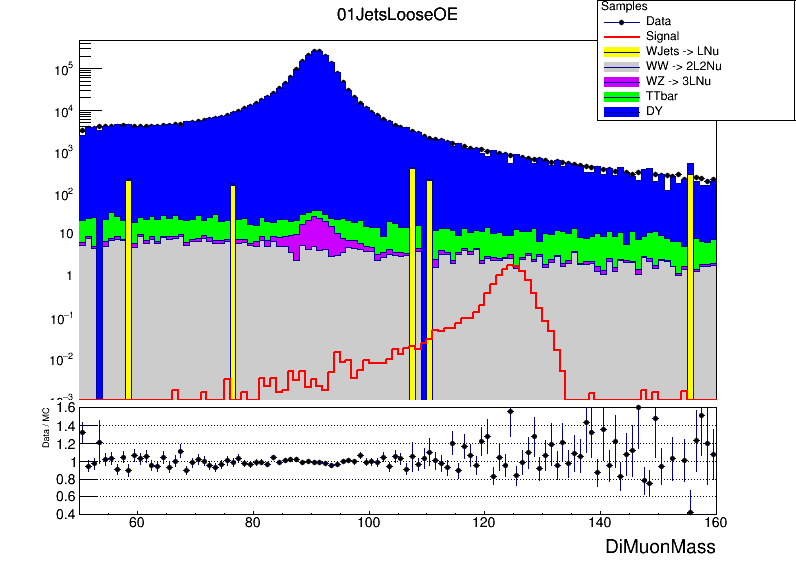
\includegraphics[width=0.65\linewidth]{figures/ch_higgs/distributions/baseline_kalman/distribution__01JetsLooseOE__DiMuonMass__logY.png}\\
  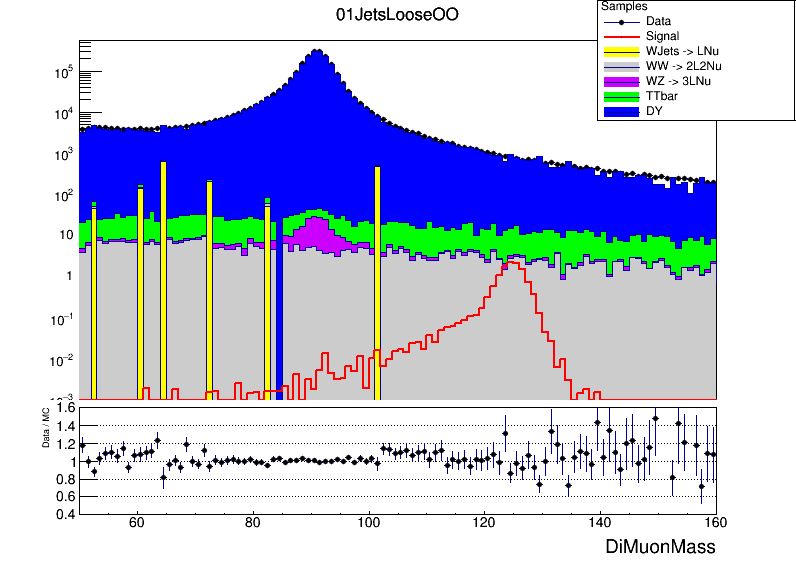
\includegraphics[width=0.65\linewidth]{figures/ch_higgs/distributions/baseline_kalman/distribution__01JetsLooseOO__DiMuonMass__logY.png}
  \caption{Mass Distributions 01JetsLooseEE (Top), 01JetsLooseOE (Middle) and 01JetsLooseOO (Bottom) Categories.}
  \label{fig:higgs_categorization_01jetslooseeeeooo}
\end{figure}

\subsection{Greedy Categorization} \label{bdt_training}
Another approach taken was to optimize the manually constructed categorization tree, discussed in the previous section, in a more systematic way by, first, training and applying a Boosted Decision Tree (BDT) for the purpose of signal to background discrimination. Then, use the BDT ouput as a new input feature for optimizing the categorization tree using a greedy optimization procedure.

In the first step, the BDT for the signal to background discrimination has been trained using both signal and background Monte Carlo samples. The BDT implementation from the {\sc ROOT}~\cite{ROOT} framework has been successfully used. Given that background samples are not utilized for the statistical analysis, all of the available MC background events are employed for the purpose of training, cross-validation and testing. However, in terms of the Higgs signal, the even-numbered events are used for the categorization optimization. The rest is reserved for the statistical analysis. The following kinematic variables are used as input features for the BDT:
\begin{itemize}
  \item The $p_t^{\mu\mu}$ of the dimuon system
  \item The $\eta_{\mu\mu}$ of the dimuon system.
  \item The $|\Delta \eta|$ between the muons from the Higgs candidate.
  \item The $|\Delta \phi|$ between the muons from the Higgs candidate.
  \item The $\eta_{jj}$ of the dijet system. 2 highest $p_t$ jets are used.
  \item The $m_{jj}$ of the dijet system. 2 highest $p_t$ jets are used.
  \item The $|\Delta \eta|$ between the 2 highest $p_t$ jets.
  \item The number of Central jets with $|\eta| < 2.4$
  \item The number of Forward jets with $|\eta| > 2.4$
  \item The number of b-tagged jets - jets passing the CSVv2 medium b-tag working point
  \item The \MET
\end{itemize}
As it follows from the above list, there is no dependence on the Higgs candidate mass among the features. In other words, given the above features, one can not deduce the mass value of the dimuon system. Mass independence is an importan tcriteria of this discrimination technique.

After the training and cross-validation to tune the hyper parameters of the decision tree itself, the results for the test dataset are shown in figure~\ref{fig:higgs_categorization_bdtoutputroc}, where the BDT ouput distributions for both training and testing subsets are overlaid and are in a very good agreement. Furthermore, the ROC curve from figure~\ref{fig:higgs_categorization_bdtoutputroc}, which is an indicator of the efficiency of the selection and rejection at the same time, shows a definite deviation from the diagonal (no discrimination). It follows that even with 0 \% efficiency rejecting background, the signal classification is not 100 \% efficient. Finally, given that a pure binary classficiation is not performed, the BDT output score is preserved for the next stage.
\begin{figure}[htbp]
  \centering
  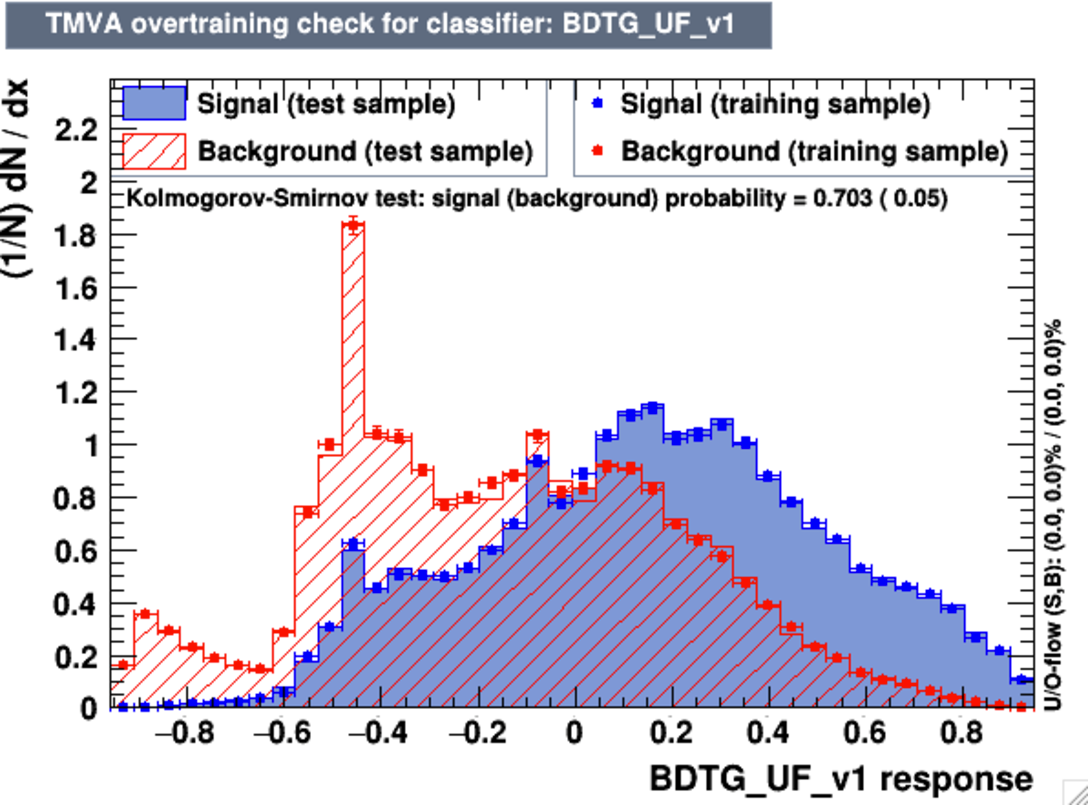
\includegraphics[width=0.75\linewidth]{figures/bdt_training/BDT_out_ge0j_all.pdf}\\
  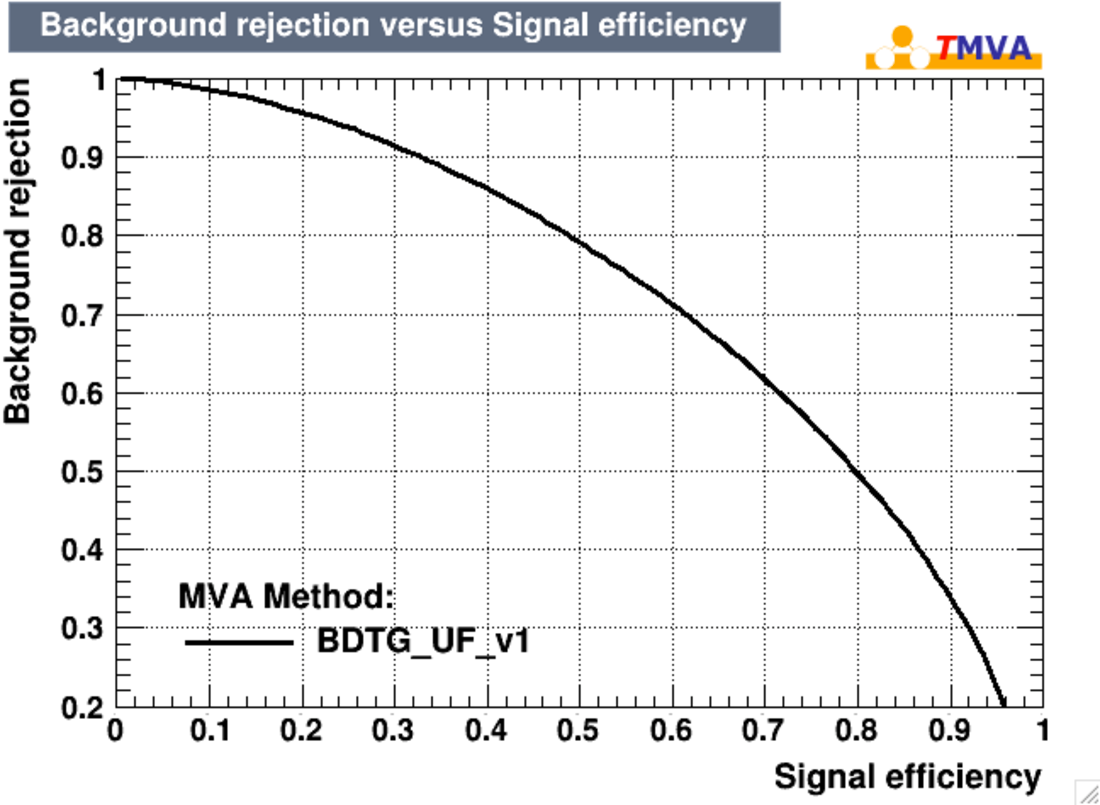
\includegraphics[width=0.75\linewidth]{figures/bdt_training/BDT_ROC_ge0j_all.pdf}
  \caption{BDT score distribution (Top) and Receiver Operating Curve, ROC, (Bottom) - a kind of True Negative/Positive selection efficiency indicator.}
  \label{fig:higgs_categorization_bdtoutputroc}
\end{figure}

The next step of the Greedy Categorization procedure is to optimize the categorization tree selections and perform the actual splitting of events into different subsets. For that purpose, a simple decision tree is used with a custom metric, signal significance, and with the following 2 features:
\begin{itemize}
  \item max($\eta_{\mu_1}$, $\eta_{\mu_2}$) - max $\eta among the muons from the Higgs Candidate pair$
  \item Discriminting BDT score
\end{itemize}
Again, only part of the signal has been used for the training, whereas all of the background events have been passed through the custom decision tree.

Before moving forward with the actual algorithm, a few definitions are provided. First of all the objects to be used are the dimuon mass histogrammes as in figure~\ref{fig:higgs_categorization_massc0}. For a given mass distribution, define a signal significance ($S_{node}$) according to the equation~\ref{eq:higgs_categorization_significance}. $N^{S}_{c,i}$ and $N^{B}_{c,i}$ are the yields (number of entries) for that particular histogram and for that particular bin. Note that all the bins in the distribution are treated separately and only those that fall in the [120 GeV, 130 GeV] mass range are used. Futhermore, the metric, based on which the splitting is optimized, is provided in equation~\ref{eq:higgs_categorization_gain}. Roughly speaking, the split that gives the maximum gain across all of the possible splits is to be selected.
\begin{equation}
  {S^2_c} = \sum_{c,i}N^{S2}_{c,i}/N^{B}_{c,i}
  \label{eq:higgs_categorization_significance}
\end{equation}
\begin{equation}
  {G} = {S^2_{left}} + {S^2_{right}} - {S^2_{node}}
  \label{eq:higgs_categorization_gain}
\end{equation}
\begin{figure}[htbp]
  \centering
  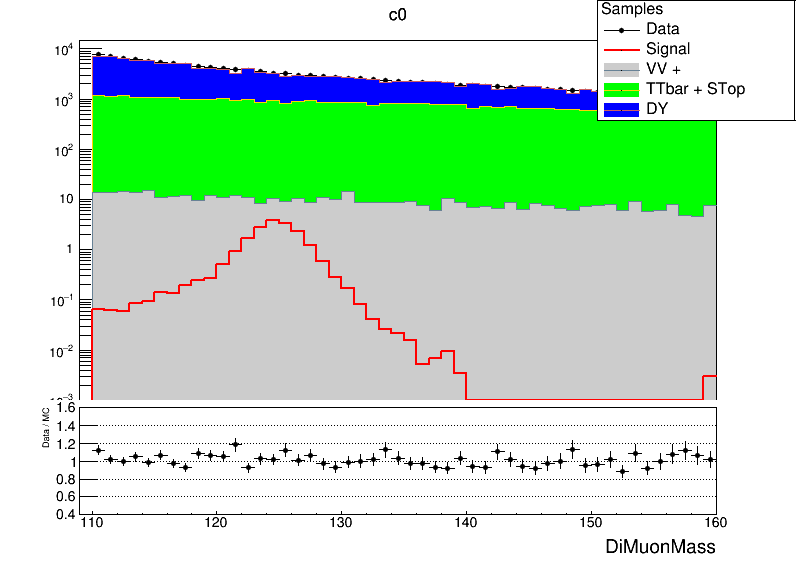
\includegraphics[width=0.9\linewidth]{figures/ch_higgs/distributions/bdt_uf/distribution__c0__DiMuonMass__logY.png}
  \caption{Mass Distribution for Category ''c0'' - lowest Discriminating BDT score category}
  \label{fig:higgs_categorization_massc0}
\end{figure}

After providing all of the important definitions to work with, the actual procedure for the tree splits optimization can be summarized as follows:
\begin{itemize}
  \item Stage 1. Start out with the inclusive set of all events - a node.
  \item Stage 2. Greedily scan through the features and select the split:
    \begin{itemize}
      \item Scan through all of the possible values of max($\eta_{\mu_1}$, $\eta_{\mu_2}$) as split's candidates. Save the split that produces maximum gain.
      \item Scan through all of the possible values of the BDT score. Again, save the split that maximizes the gain for the second feature.
      \item Select the split which maximizes the gain: max(G$_\eta$, G$_{score}$)
    \end{itemize}
  \item Stage n. Repeat Stage 2 recursively for each of the new nodes until the tree reaches the limit on the number of categories or runs out of splitting conditions.
\end{itemize}
The procedure just described is an example of a greedy algorithm, because full parameters' phase space optimization is not performed as it is computationally infeasible. Rather, the metric of interest is optimized greedily, step by step iterating over all of the available features.

The outcome of this technique is 13 new categories with the categorization tree shown in figure~\ref{fig:higgs_categorization_bdtcategories}. Integer labels are assigned based on the trained sensitivity of a particular subset, going from the category with the lowest sensitivity, ''c0'', to the one with the highest, ''c12''.
\begin{figure}[hbtp]
  \centering
  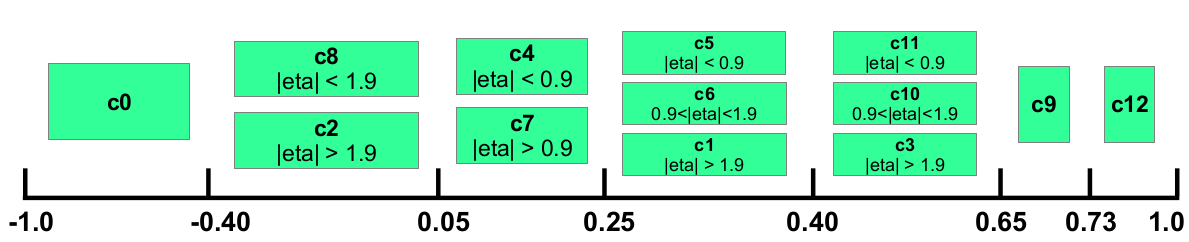
\includegraphics[width=1.0\linewidth]{figures/bdt_cats/final_categories.png}
  \caption
   {Greedy Categorization Tree.}
  \label{fig:higgs_categorization_bdtcategories}
\end{figure}

Figures~\ref{fig:higgs_categorization_greedyc1c3}-~\ref{fig:higgs_categorization_greedyc10c12} summarize the resulting dimuon mass distributions. The modeling of the dimuon mass agrees well between data and simulations.
\begin{figure}[htbp]
  \centering
  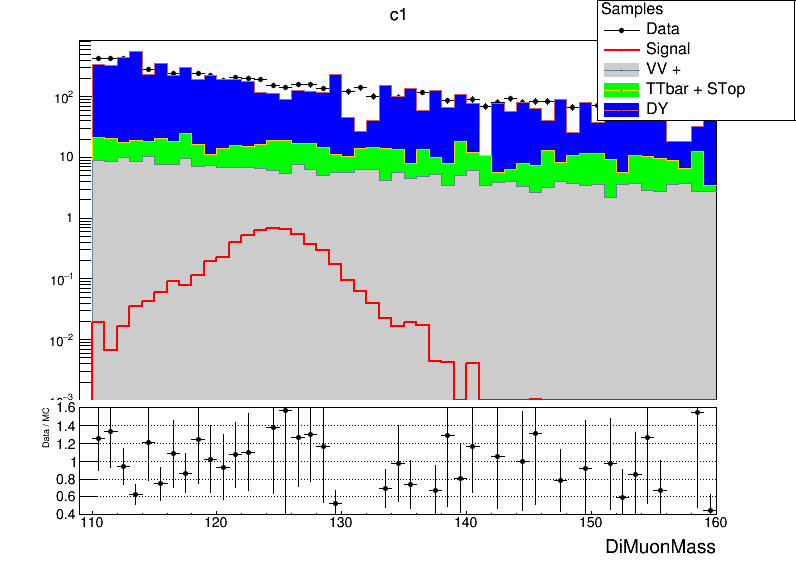
\includegraphics[width=0.65\linewidth]{figures/ch_higgs/distributions/bdt_uf/distribution__c1__DiMuonMass__logY.png}\\
  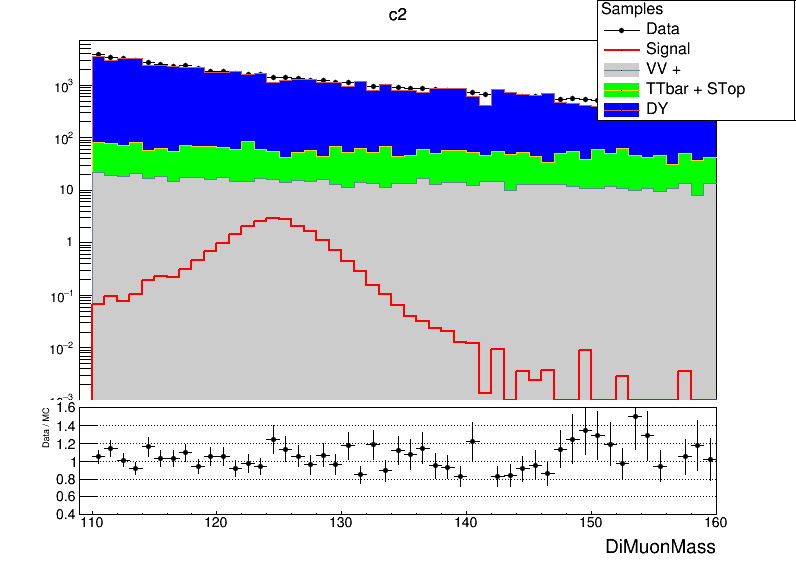
\includegraphics[width=0.65\linewidth]{figures/ch_higgs/distributions/bdt_uf/distribution__c2__DiMuonMass__logY.png}\\
  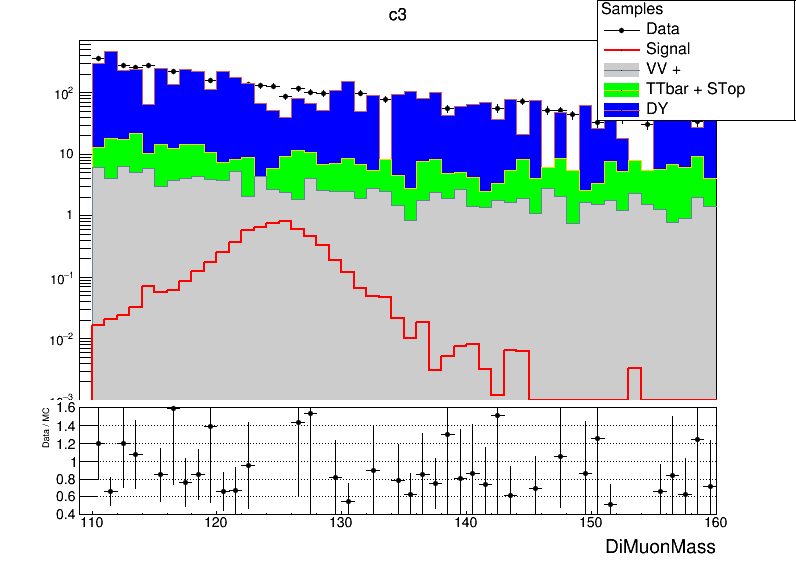
\includegraphics[width=0.65\linewidth]{figures/ch_higgs/distributions/bdt_uf/distribution__c3__DiMuonMass__logY.png}
  \caption{Mass Distributions for c1-c3 subsets from the Greedy Categorization}
  \label{fig:higgs_categorization_greedyc1c3}
\end{figure}
\begin{figure}[htbp]
  \centering
  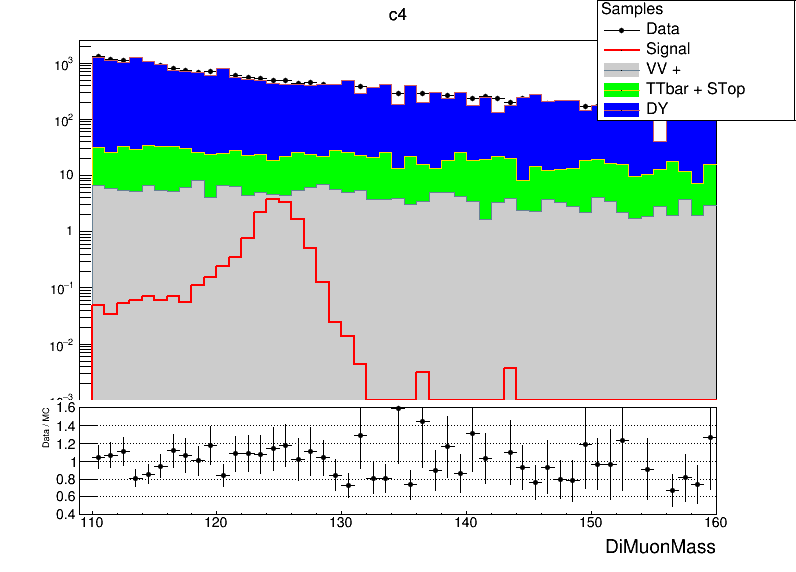
\includegraphics[width=0.65\linewidth]{figures/ch_higgs/distributions/bdt_uf/distribution__c4__DiMuonMass__logY.png}\\
  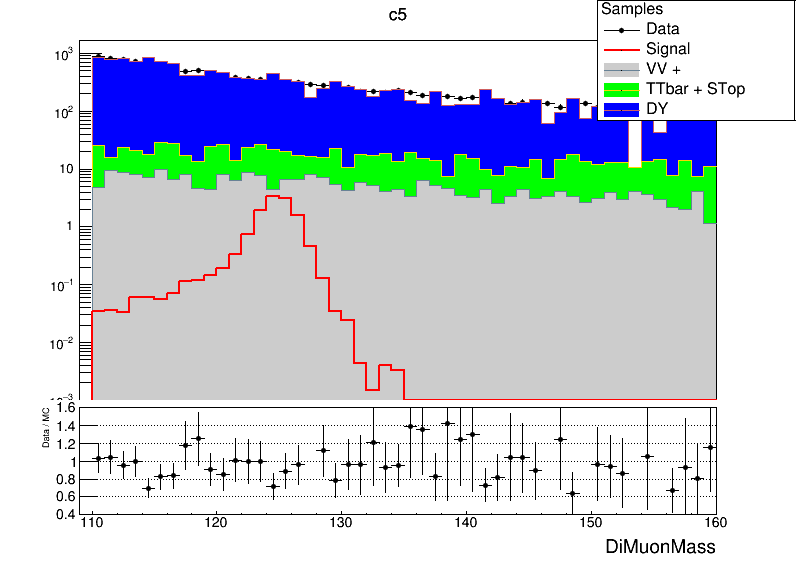
\includegraphics[width=0.65\linewidth]{figures/ch_higgs/distributions/bdt_uf/distribution__c5__DiMuonMass__logY.png}\\
  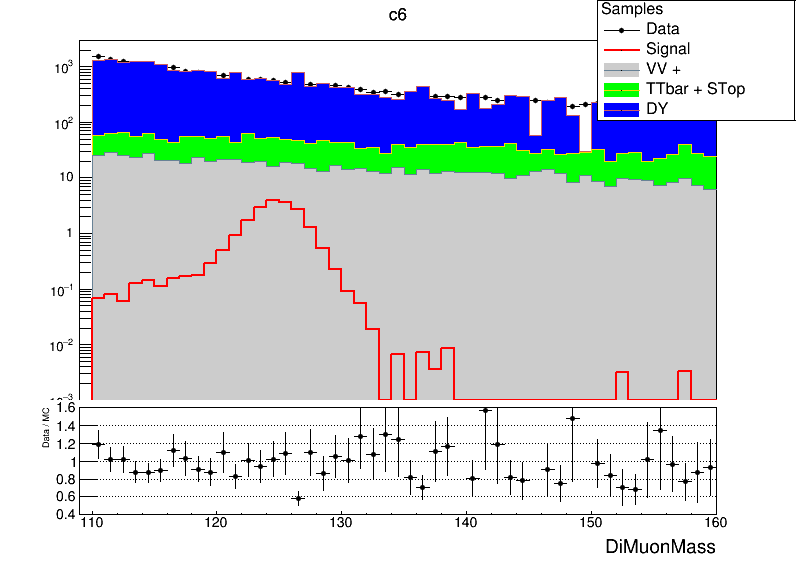
\includegraphics[width=0.65\linewidth]{figures/ch_higgs/distributions/bdt_uf/distribution__c6__DiMuonMass__logY.png}
  \caption{Msas Distributions for c4-c6 subsets from the Greedy Categorization}
  \label{fig:higgs_categorization_greedyc4c6}
\end{figure}
\begin{figure}[htbp]
  \centering
  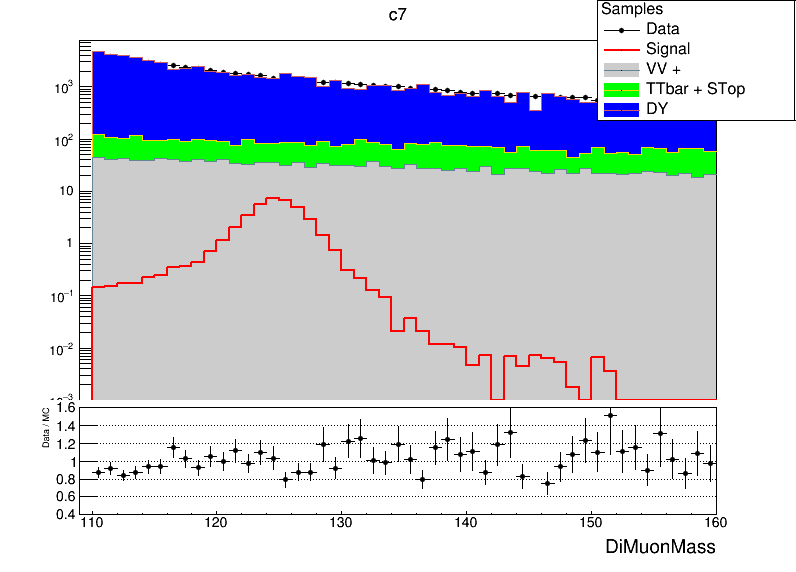
\includegraphics[width=0.65\linewidth]{figures/ch_higgs/distributions/bdt_uf/distribution__c7__DiMuonMass__logY.png}\\
  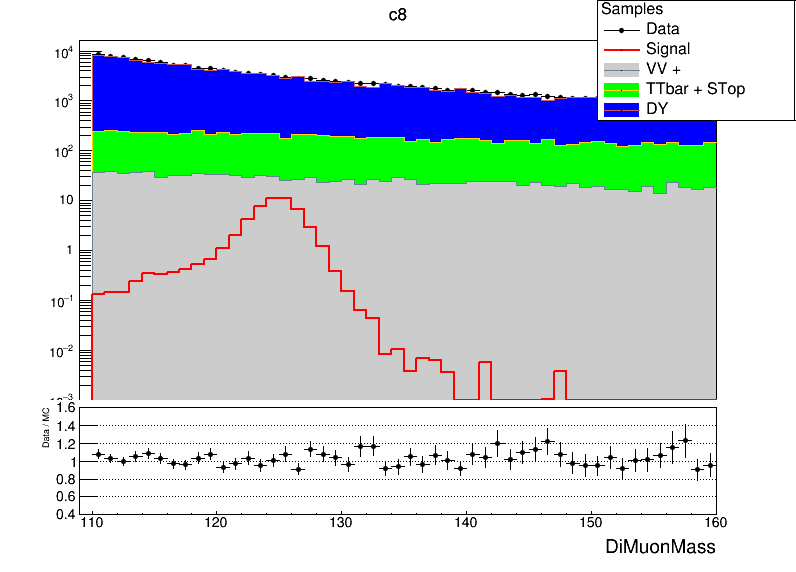
\includegraphics[width=0.65\linewidth]{figures/ch_higgs/distributions/bdt_uf/distribution__c8__DiMuonMass__logY.png}\\
  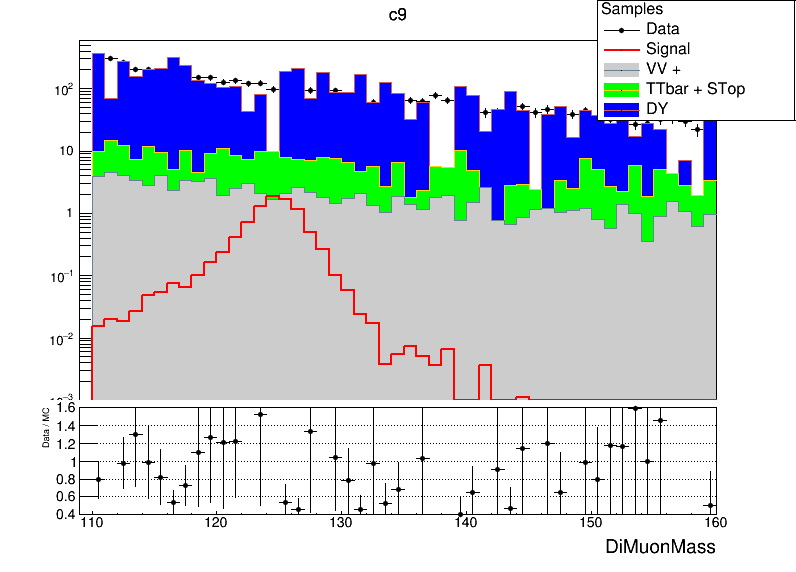
\includegraphics[width=0.65\linewidth]{figures/ch_higgs/distributions/bdt_uf/distribution__c9__DiMuonMass__logY.png}
  \caption{Mass Distributions for c7-c9 subsets from the Greedy Categorization}
  \label{fig:higgs_categorization_greedyc7c9}
\end{figure}
\begin{figure}[htbp]
  \centering
  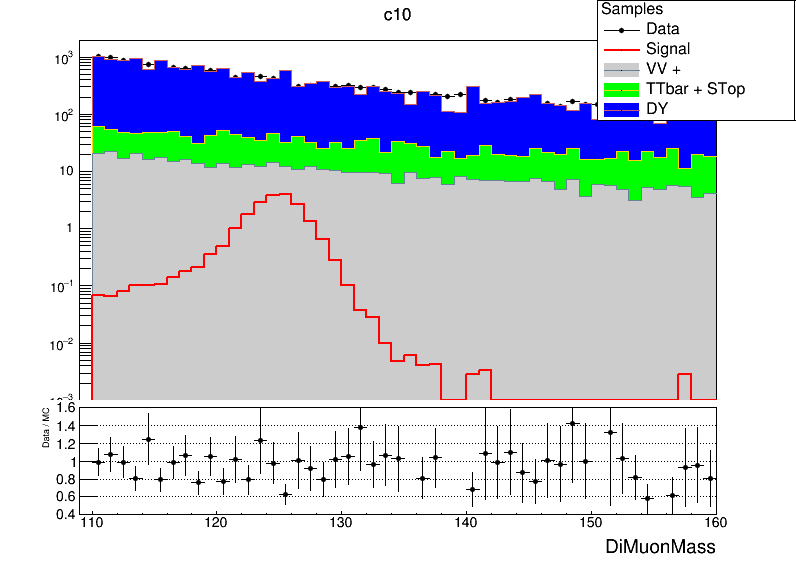
\includegraphics[width=0.65\linewidth]{figures/ch_higgs/distributions/bdt_uf/distribution__c10__DiMuonMass__logY.png}\\
  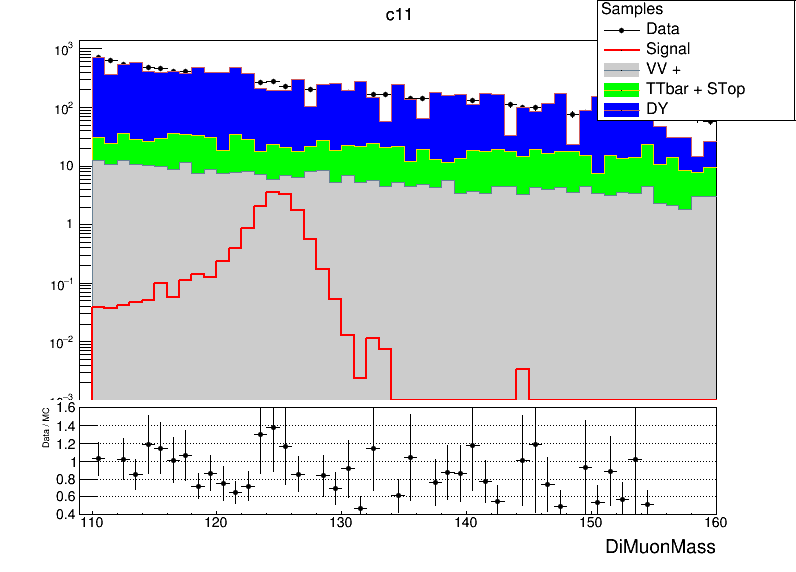
\includegraphics[width=0.65\linewidth]{figures/ch_higgs/distributions/bdt_uf/distribution__c11__DiMuonMass__logY.png}\\
  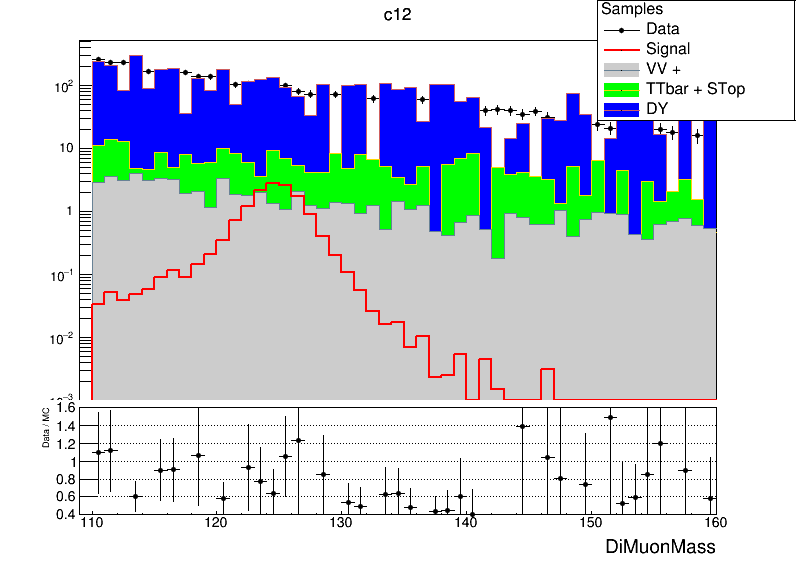
\includegraphics[width=0.65\linewidth]{figures/ch_higgs/distributions/bdt_uf/distribution__c12__DiMuonMass__logY.png}
  \caption{Mass Distributions for c10-c12 subsets fomr the Greedy Categorization}
  \label{fig:higgs_categorization_greedyc10c12}
\end{figure}

Figures~\ref{fig:higgs_categorization_bdtinput1_inclusive},~\ref{fig:higgs_categorization_bdtinput2_inclusive} provide a comparison of the data with MC for the kinematic variables, input features, that are used for the signal discrimination. Figures~\ref{fig:higgs_categorization_bdtinput1_c12},~\ref{fig:higgs_categorization_bdtinput2_c12} show the same features but compared for the most sensitive category, ''c12''. Overall, good agreement between data and simulations is observed, especially for the dimuon mass distributions.
\begin{figure}[htbp]
  \centering
  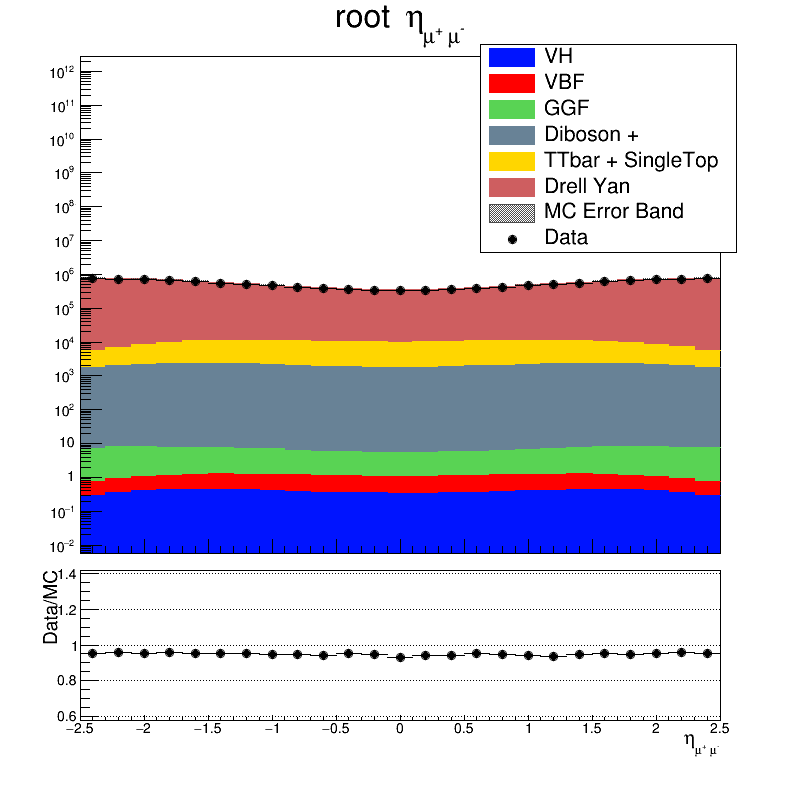
\includegraphics[width=0.49\linewidth]{figures/bdt_cats/dimu_eta_root.png}
  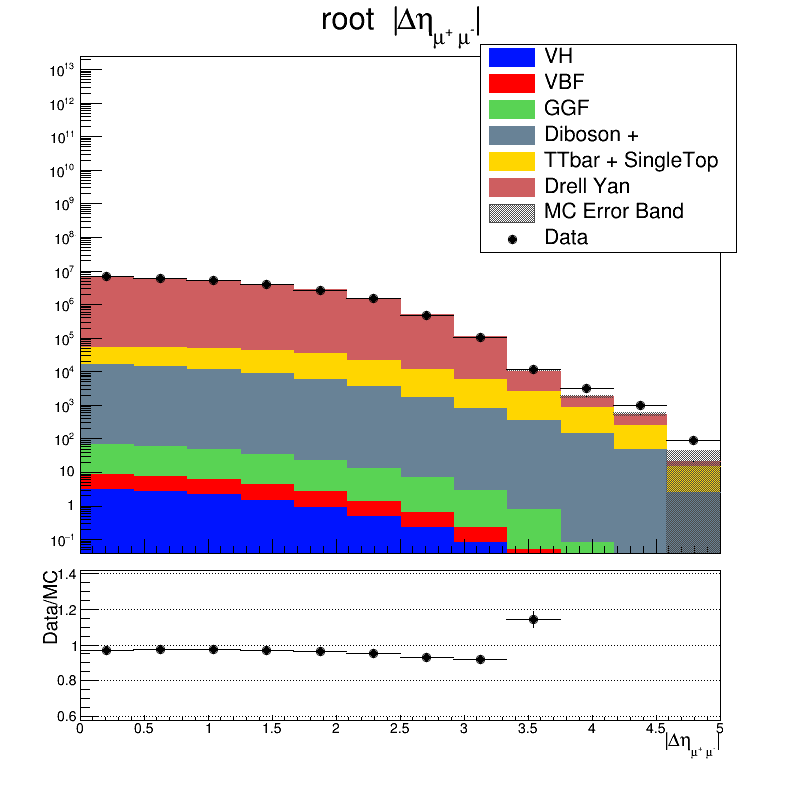
\includegraphics[width=0.49\linewidth]{figures/bdt_cats/dimu_abs_dEta_root.png}\\
  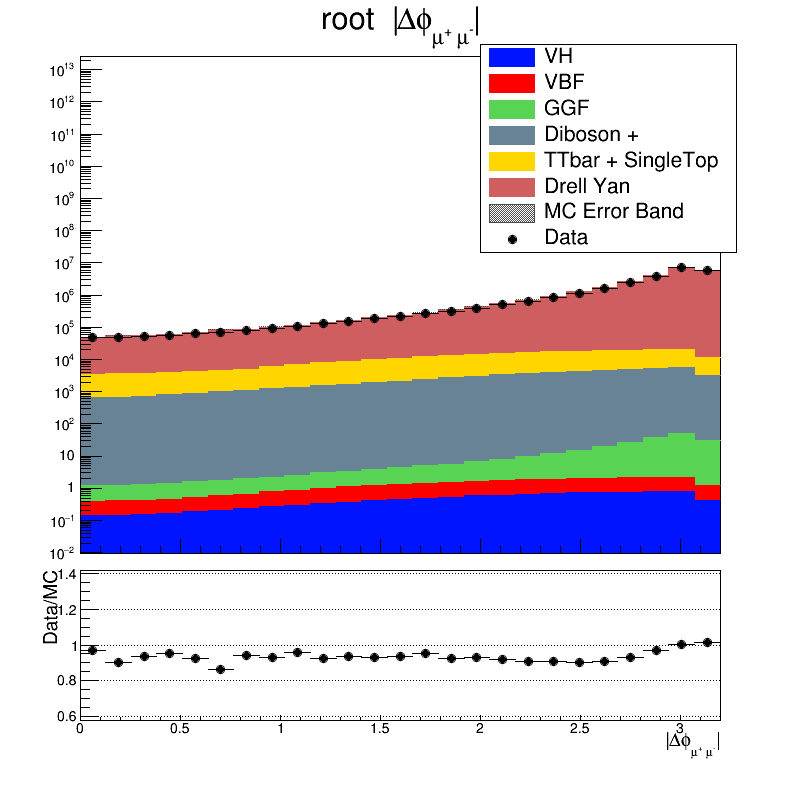
\includegraphics[width=0.49\linewidth]{figures/bdt_cats/dimu_abs_dPhi_root.png}
  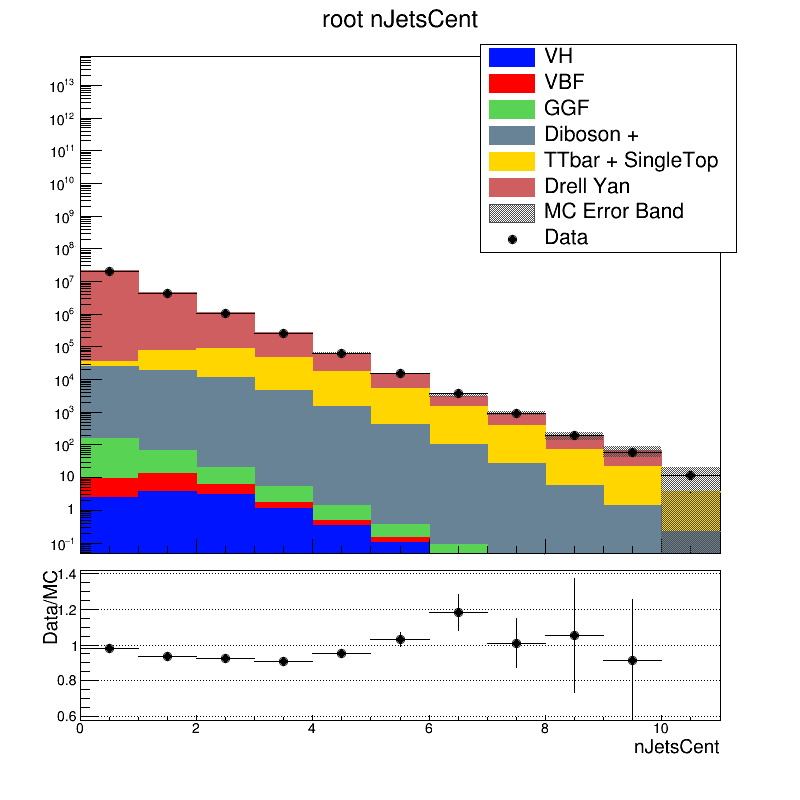
\includegraphics[width=0.49\linewidth]{figures/bdt_cats/nJetsCent_root.png}
  \caption{Data/MC agreement for the BDT input variables before categorization.}
  \label{fig:higgs_categorization_bdtinput1_inclusive}
\end{figure}

\begin{figure}[htbp]
  \centering
  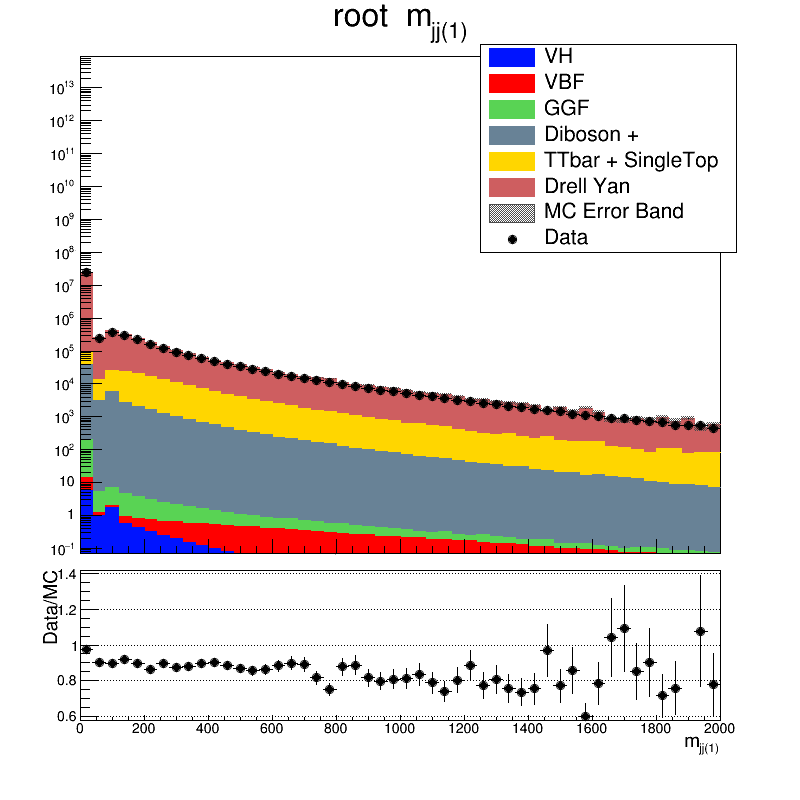
\includegraphics[width=0.49\linewidth]{figures/bdt_cats/dijet1_mass_root.png}
  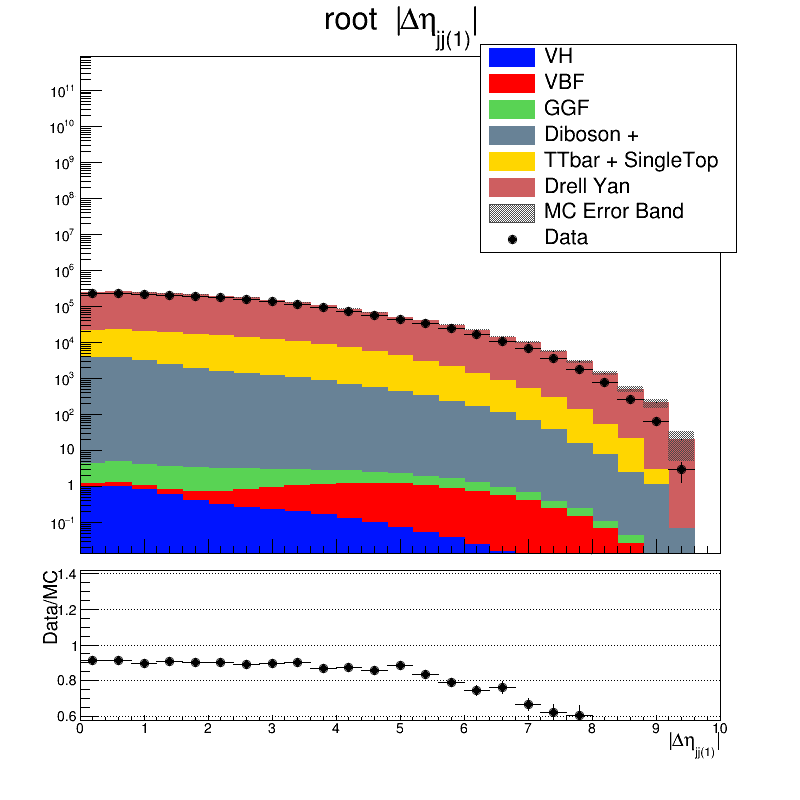
\includegraphics[width=0.49\linewidth]{figures/bdt_cats/dijet1_abs_dEta_root.png}\\
  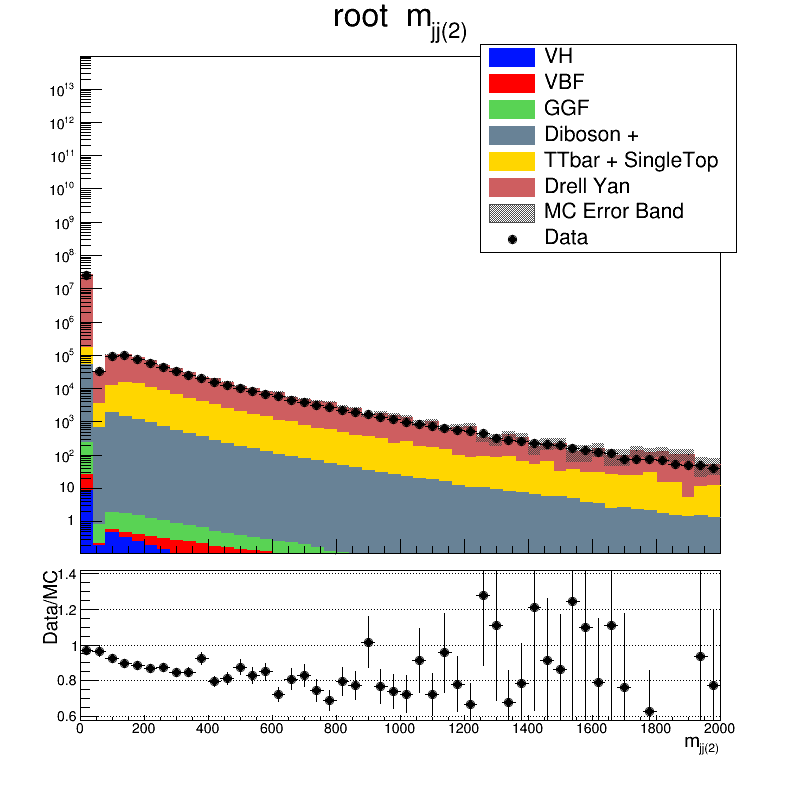
\includegraphics[width=0.49\linewidth]{figures/bdt_cats/dijet2_mass_root.png}
  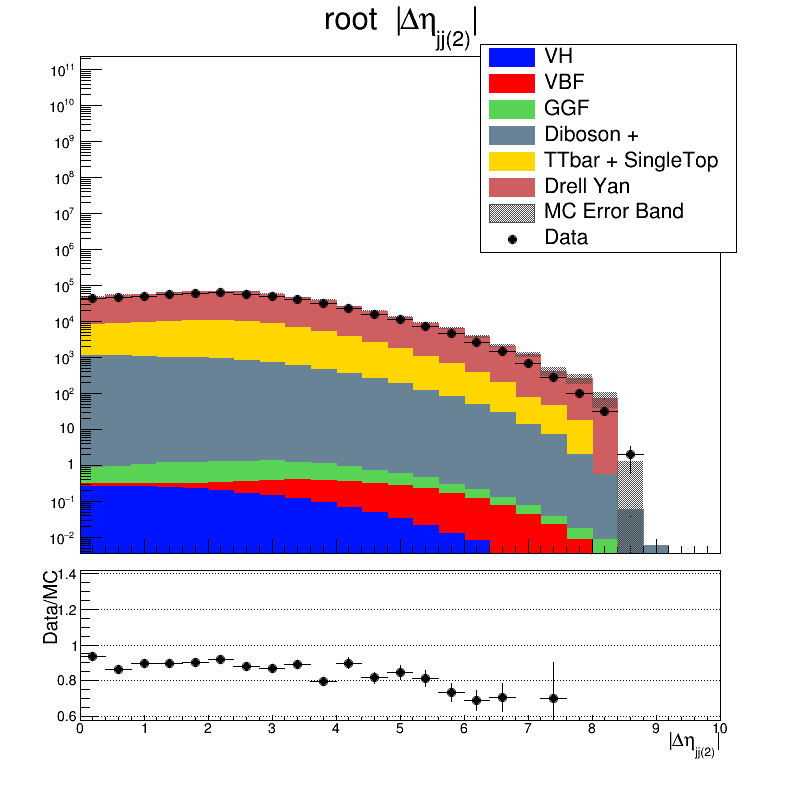
\includegraphics[width=0.49\linewidth]{figures/bdt_cats/dijet2_abs_dEta_root.png}
  \caption{Data/MC agreement for the BDT input variables before categorization.}
  \label{fig:higgs_categorization_bdtinput2_inclusive}
\end{figure}

\begin{figure}[htbp]
  \centering
  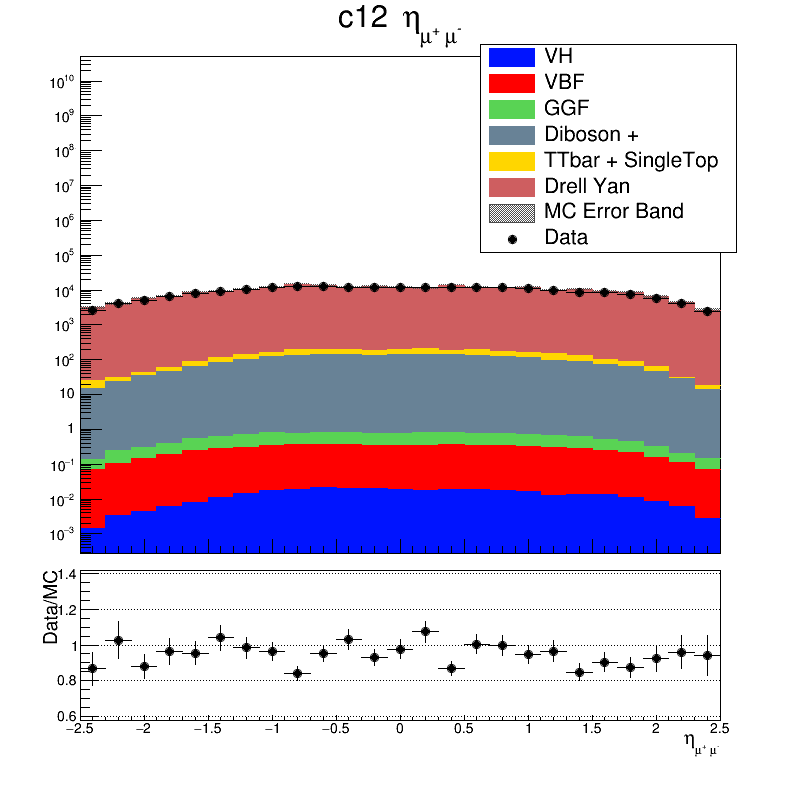
\includegraphics[width=0.49\linewidth]{figures/bdt_cats/dimu_eta_c12.png}
  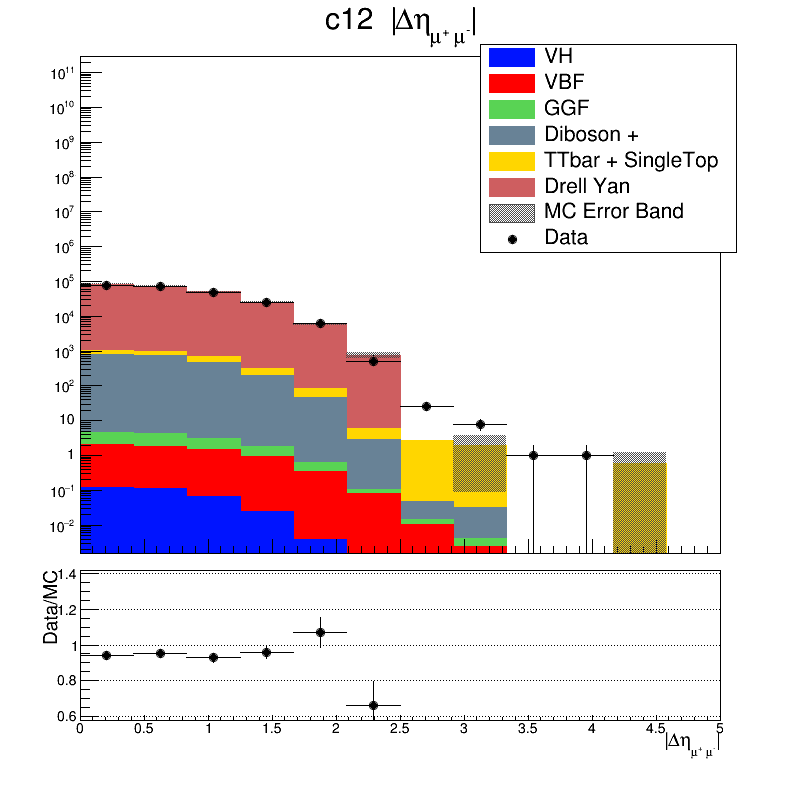
\includegraphics[width=0.49\linewidth]{figures/bdt_cats/dimu_abs_dEta_c12.png}\\
  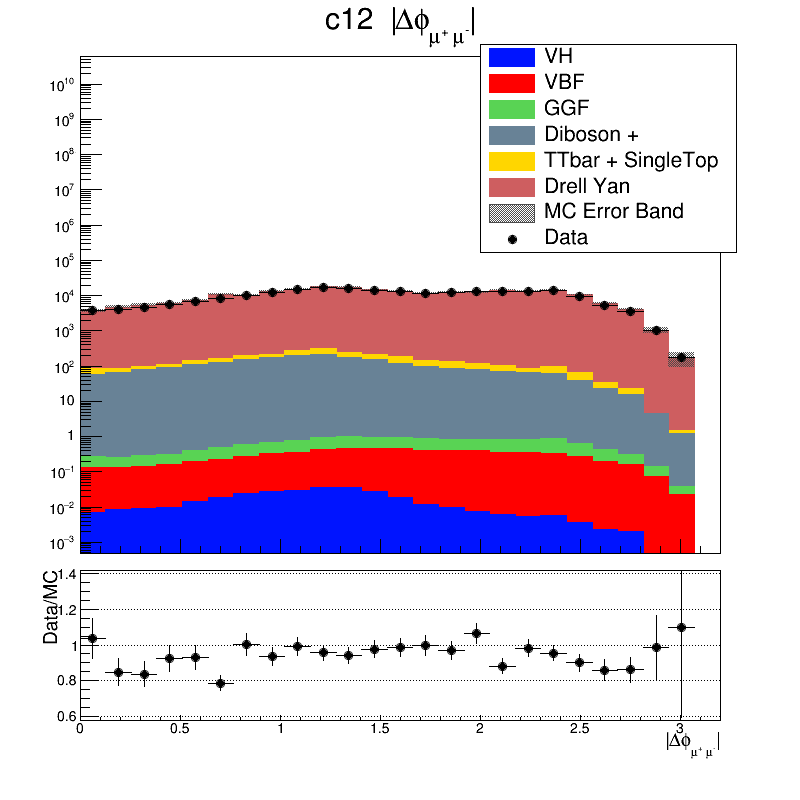
\includegraphics[width=0.49\linewidth]{figures/bdt_cats/dimu_abs_dPhi_c12.png}
  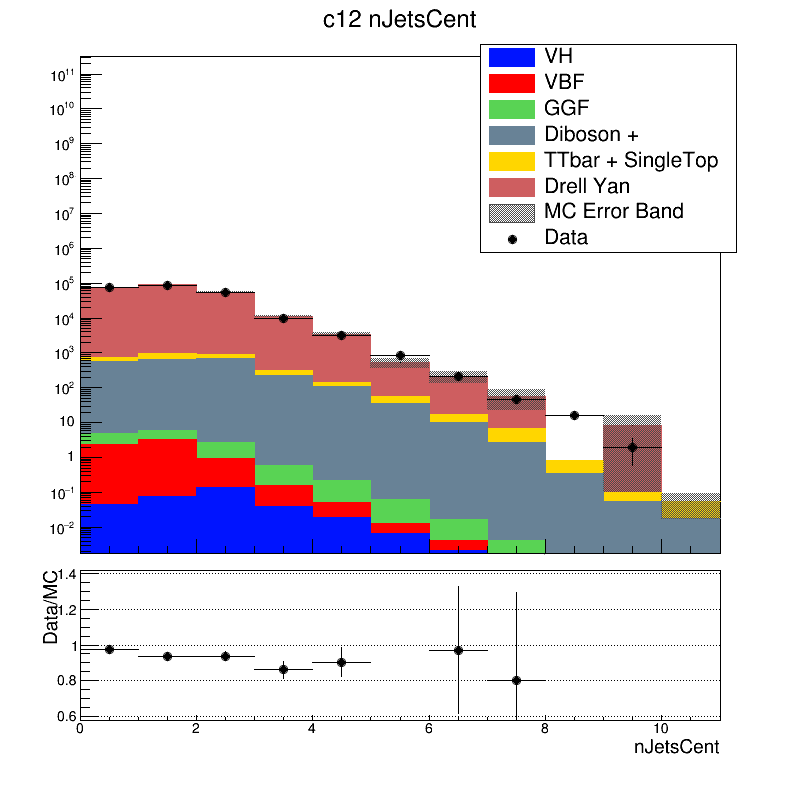
\includegraphics[width=0.49\linewidth]{figures/bdt_cats/nJetsCent_c12.png}
  \caption{Data/MC agreement for the BDT input varaibles for the most sensitive category.}
  \label{fig:higgs_categorization_bdtinput1_c12}
\end{figure}

\begin{figure}[htbp]
  \centering
  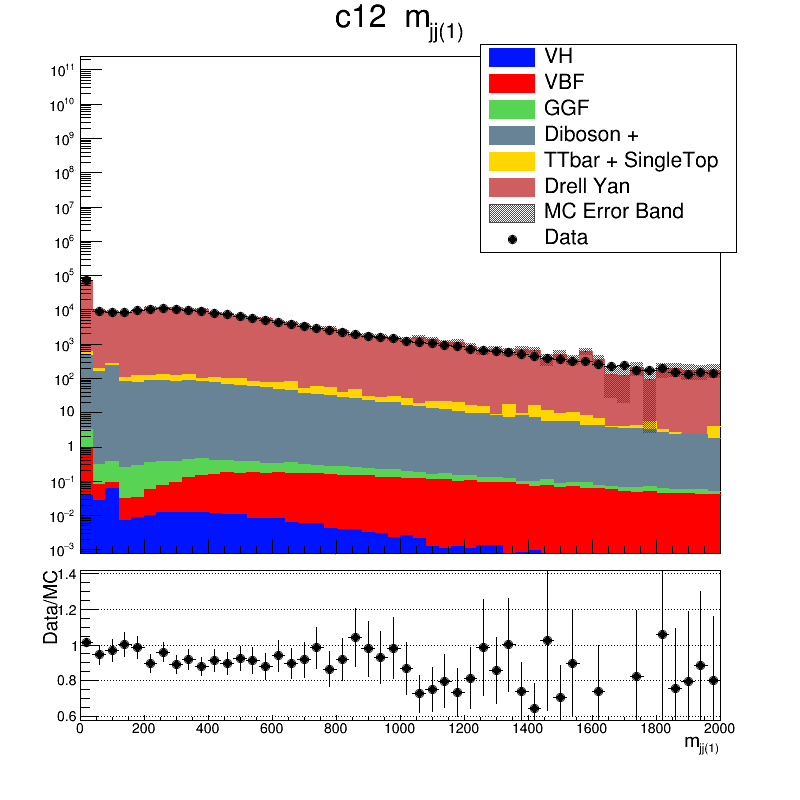
\includegraphics[width=0.49\linewidth]{figures/bdt_cats/dijet1_mass_c12.png}
  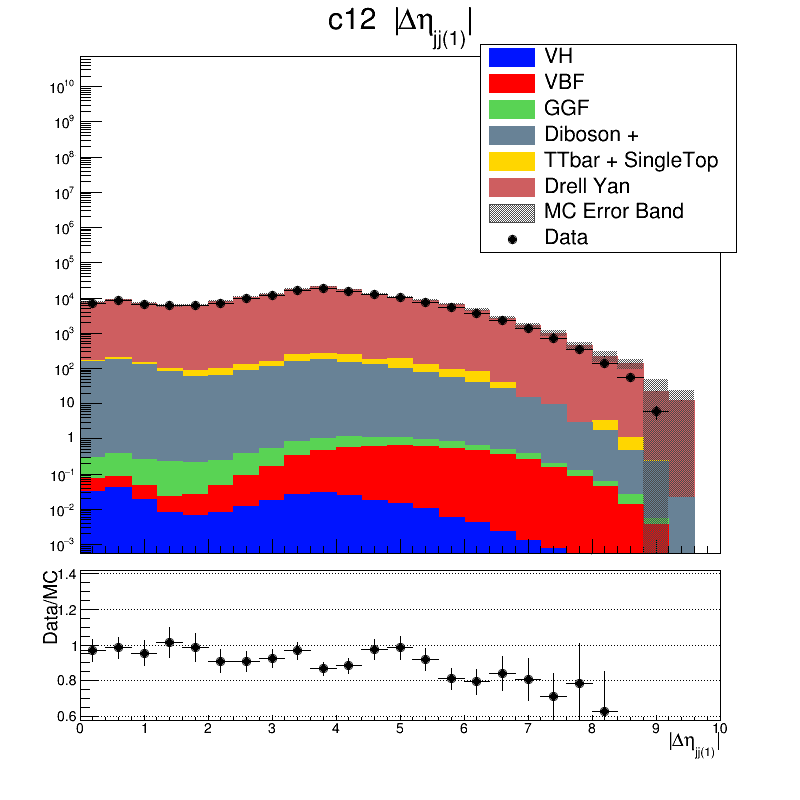
\includegraphics[width=0.49\linewidth]{figures/bdt_cats/dijet1_abs_dEta_c12.png}\\
  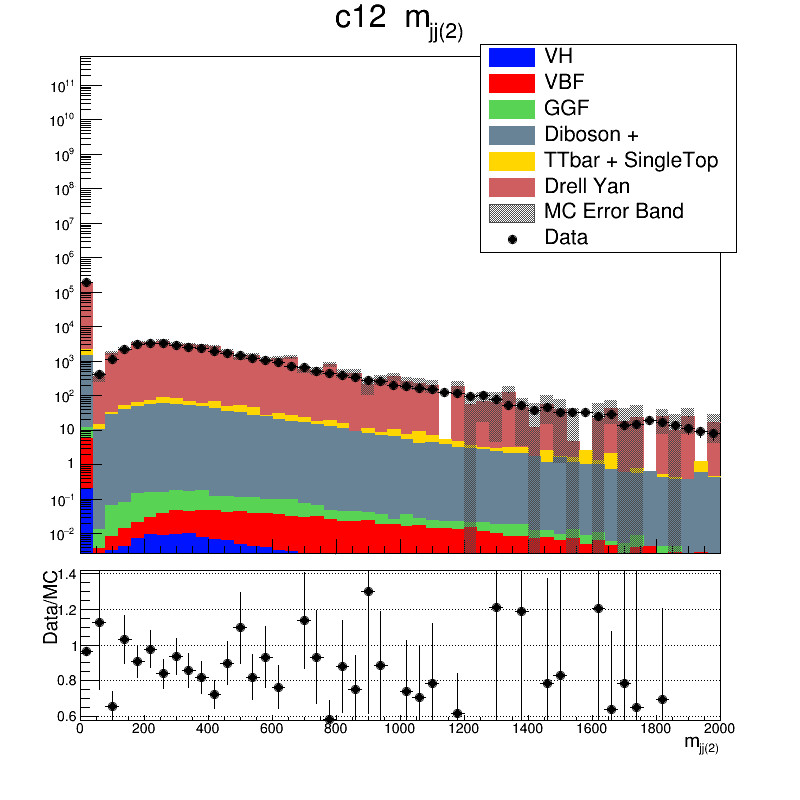
\includegraphics[width=0.49\linewidth]{figures/bdt_cats/dijet2_mass_c12.png}
  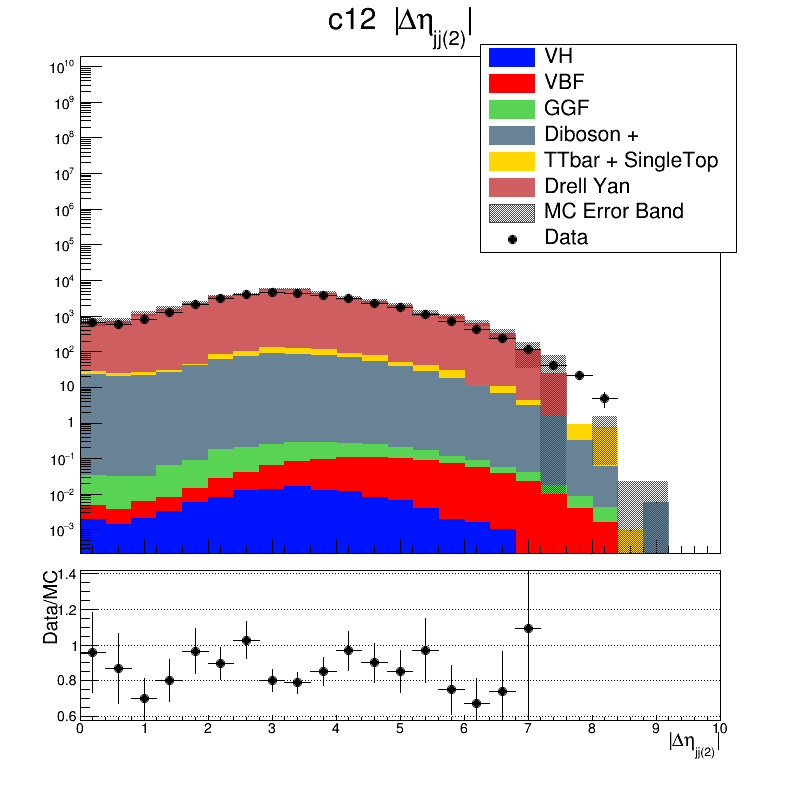
\includegraphics[width=0.49\linewidth]{figures/bdt_cats/dijet2_abs_dEta_c12.png}
  \caption{Data/MC agreement for the BDT input variables for the most sensitive category.}
  \label{fig:higgs_categorization_bdtinput2_c12}
\end{figure}

Table~\ref{tab:higgs_categorization_yields} provides a summary of the statistical properties of dimuon mass shapes provided in figures \ref{fig:higgs_categorization_greedyc1c3} - \ref{fig:higgs_categorization_greedyc10c12}. One of the important characteristics of the search, although not obvious, is the signal width, provided in terms of Full Width at Half Maximum (FWHM). It is an important feature because the smaller the width is, the more pronounced the signal is, the less influence the shape of the function, used for the background estimation, will have on the Standard Model Higgs signal.
\begin{table}[htb]
  \caption{Comparison of Signal and Background Yields for greedily optimized categories.}
  \label{tab:higgs_categorization_yields}
  \begin{center}
    \begin{tabular}{|c|c|c|c|c|c|}
      \hline
      Category  & Signal FWHM & $N^{S}$ & $N^{B}$ & $\mathrm{N^S / \sqrt{N^B}}$ \\
      \hline
      c0 & 4.4 & 13.4826 & 14187.6 & 0.113193\\
      c1 & 5.8 & 3.52888 & 970.875 & 0.113255\\
      c2 & 5.8 & 14.2112 & 8248.64 & 0.156473\\
      c3 & 6.0 & 3.82012 & 779.594 & 0.136818\\
      c4 & 3.0 & 9.92363 & 1609.08 & 0.24739\\
      c5 & 2.8 & 8.5825  & 1028.08 & 0.267671\\
      c6 & 4.0 & 14.1224 & 2371.09 & 0.290025\\
      c7 & 4.2 & 26.3575 & 6904.16 & 0.317211\\
      c8 & 3.6 & 35.6493 & 11187.4 & 0.337043\\
      c9 & 4.0 & 6.12457 & 451.281 & 0.288305\\
      c10 & 4.0 & 13.9349 & 1667.59 & 0.34124\\
      c11 & 3.0 & 9.59255 & 765.226 & 0.346768\\
      c12 & 4.0 & 9.58541 & 420.983 & 0.467173\\
      \hline
    \end{tabular}
  \end{center}
\end{table}


% \begin{figure}
%   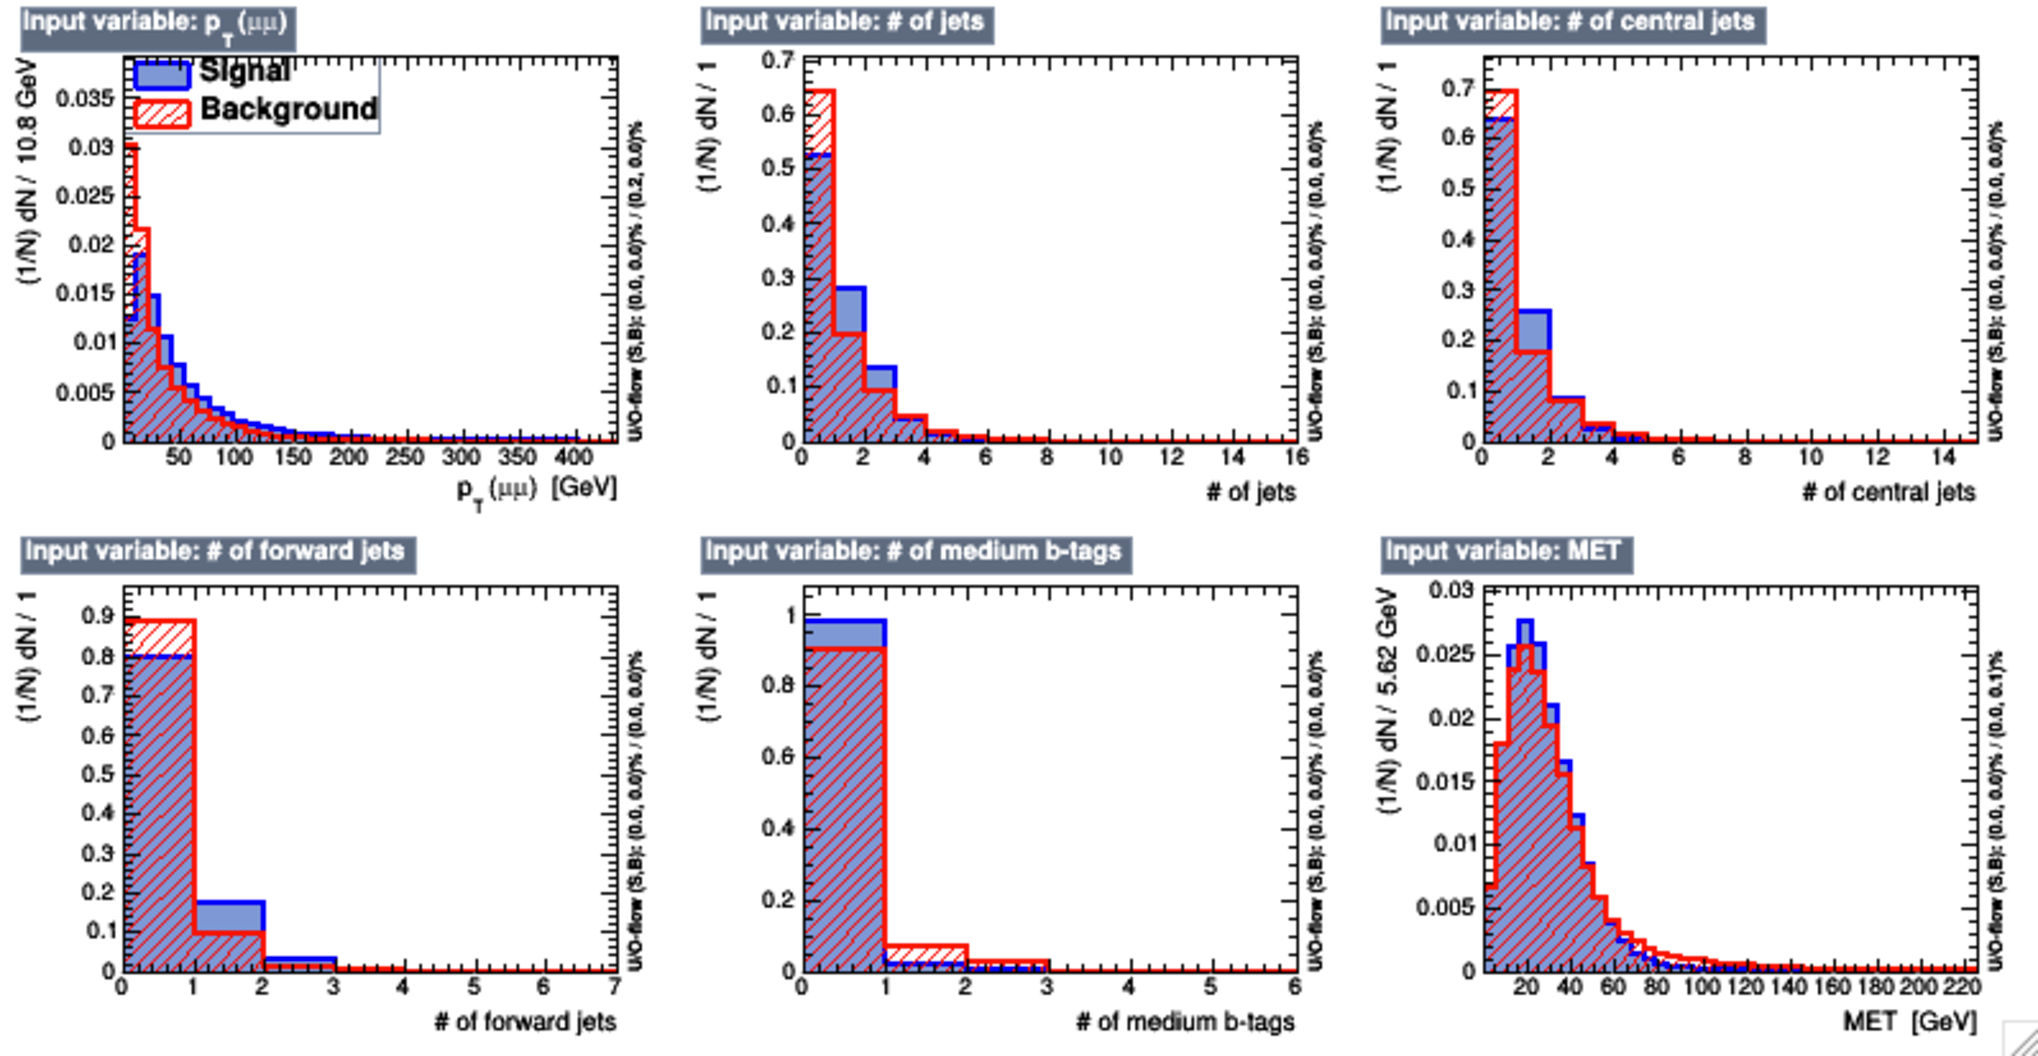
\includegraphics[width=1.0\linewidth]{figures/bdt_training/BDT_in_ge0j_all.pdf}
%   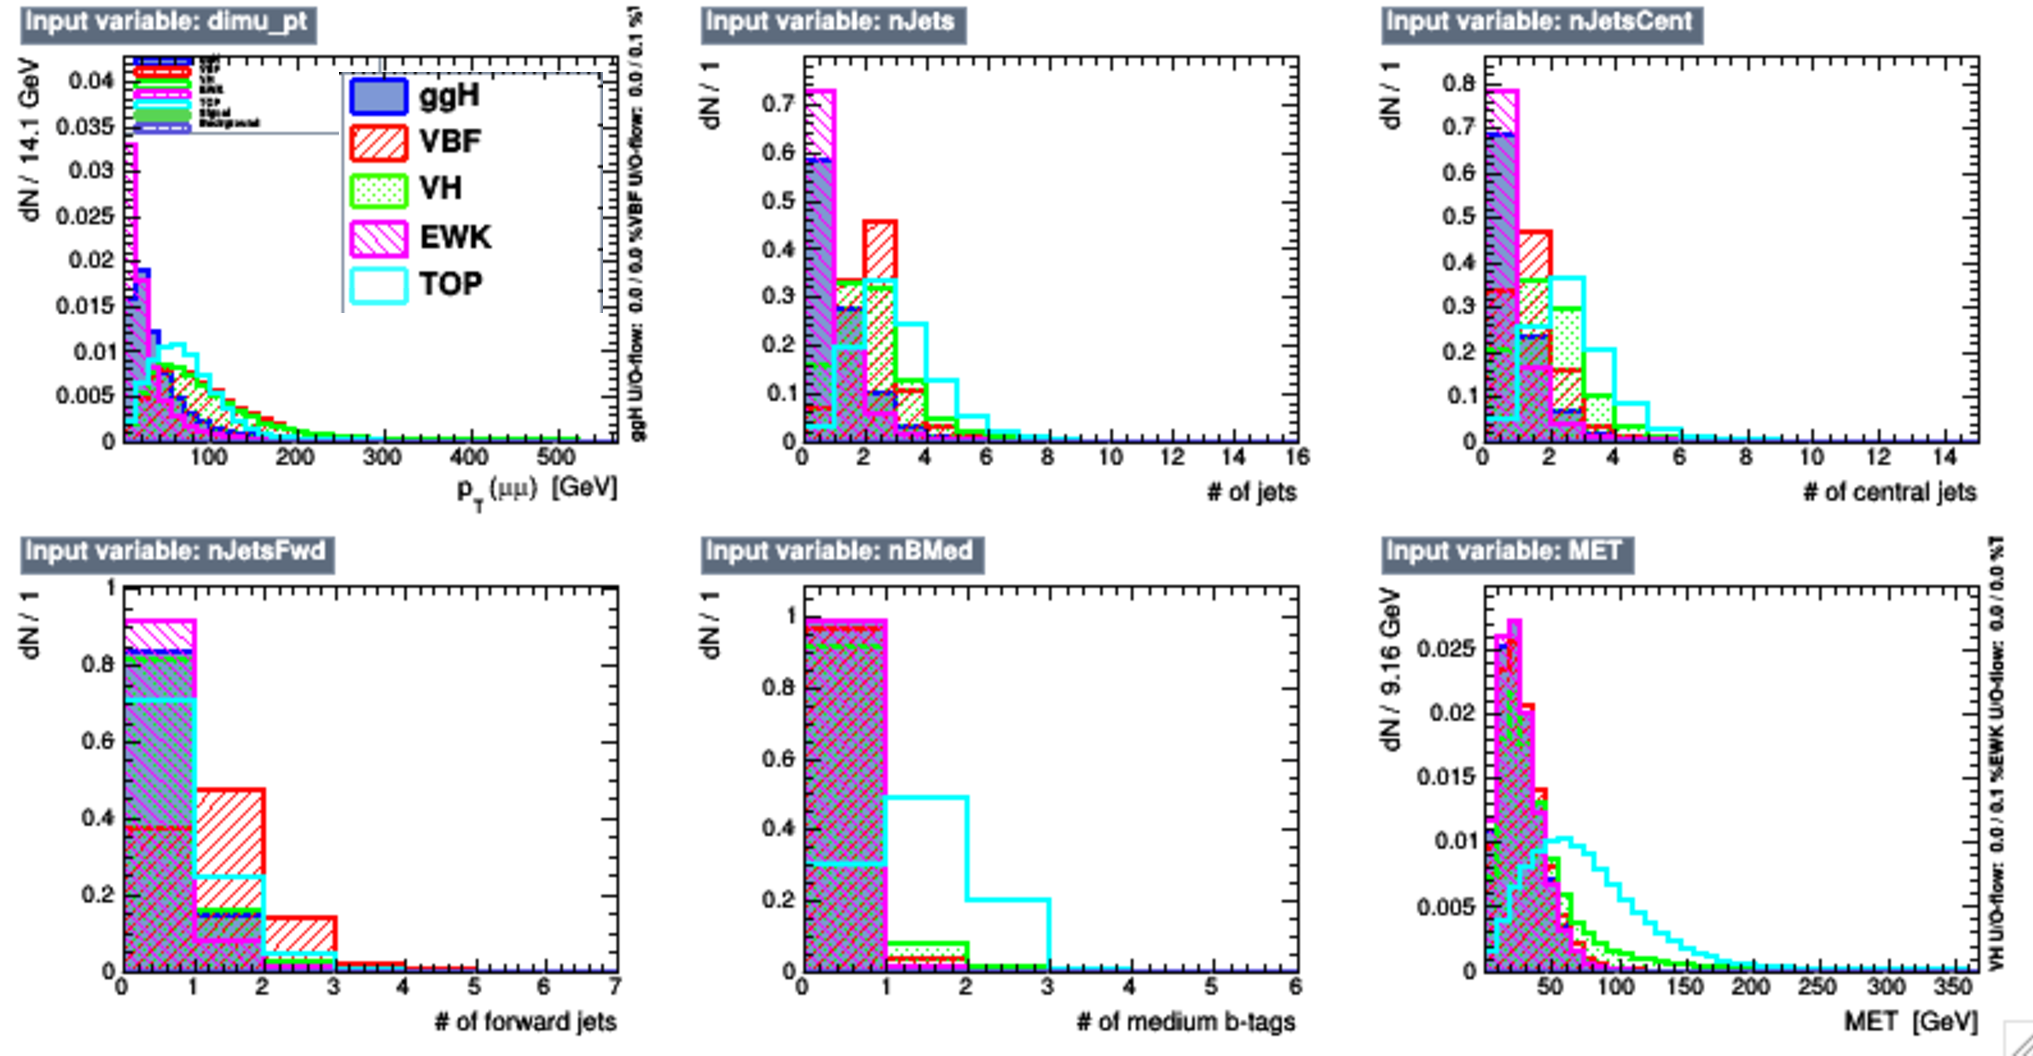
\includegraphics[width=1.0\linewidth]{figures/bdt_training/BDT_in_ge0j_sep.pdf}
%   \caption{Some BDT input variables for events with $\ge 0$ jets.
%            In the top plots, signal is in blue and background in red.
%            In the bottom plots, the gluon-fusion signal is dark blue, VBF is red, and VH is green,
%            while Drell--Yan and diboson backgrounds are pink, and \ttbar and single top are light blue.}
%   \label{fig:BDT_in_ge0j}
% \end{figure}

% \begin{figure}
%   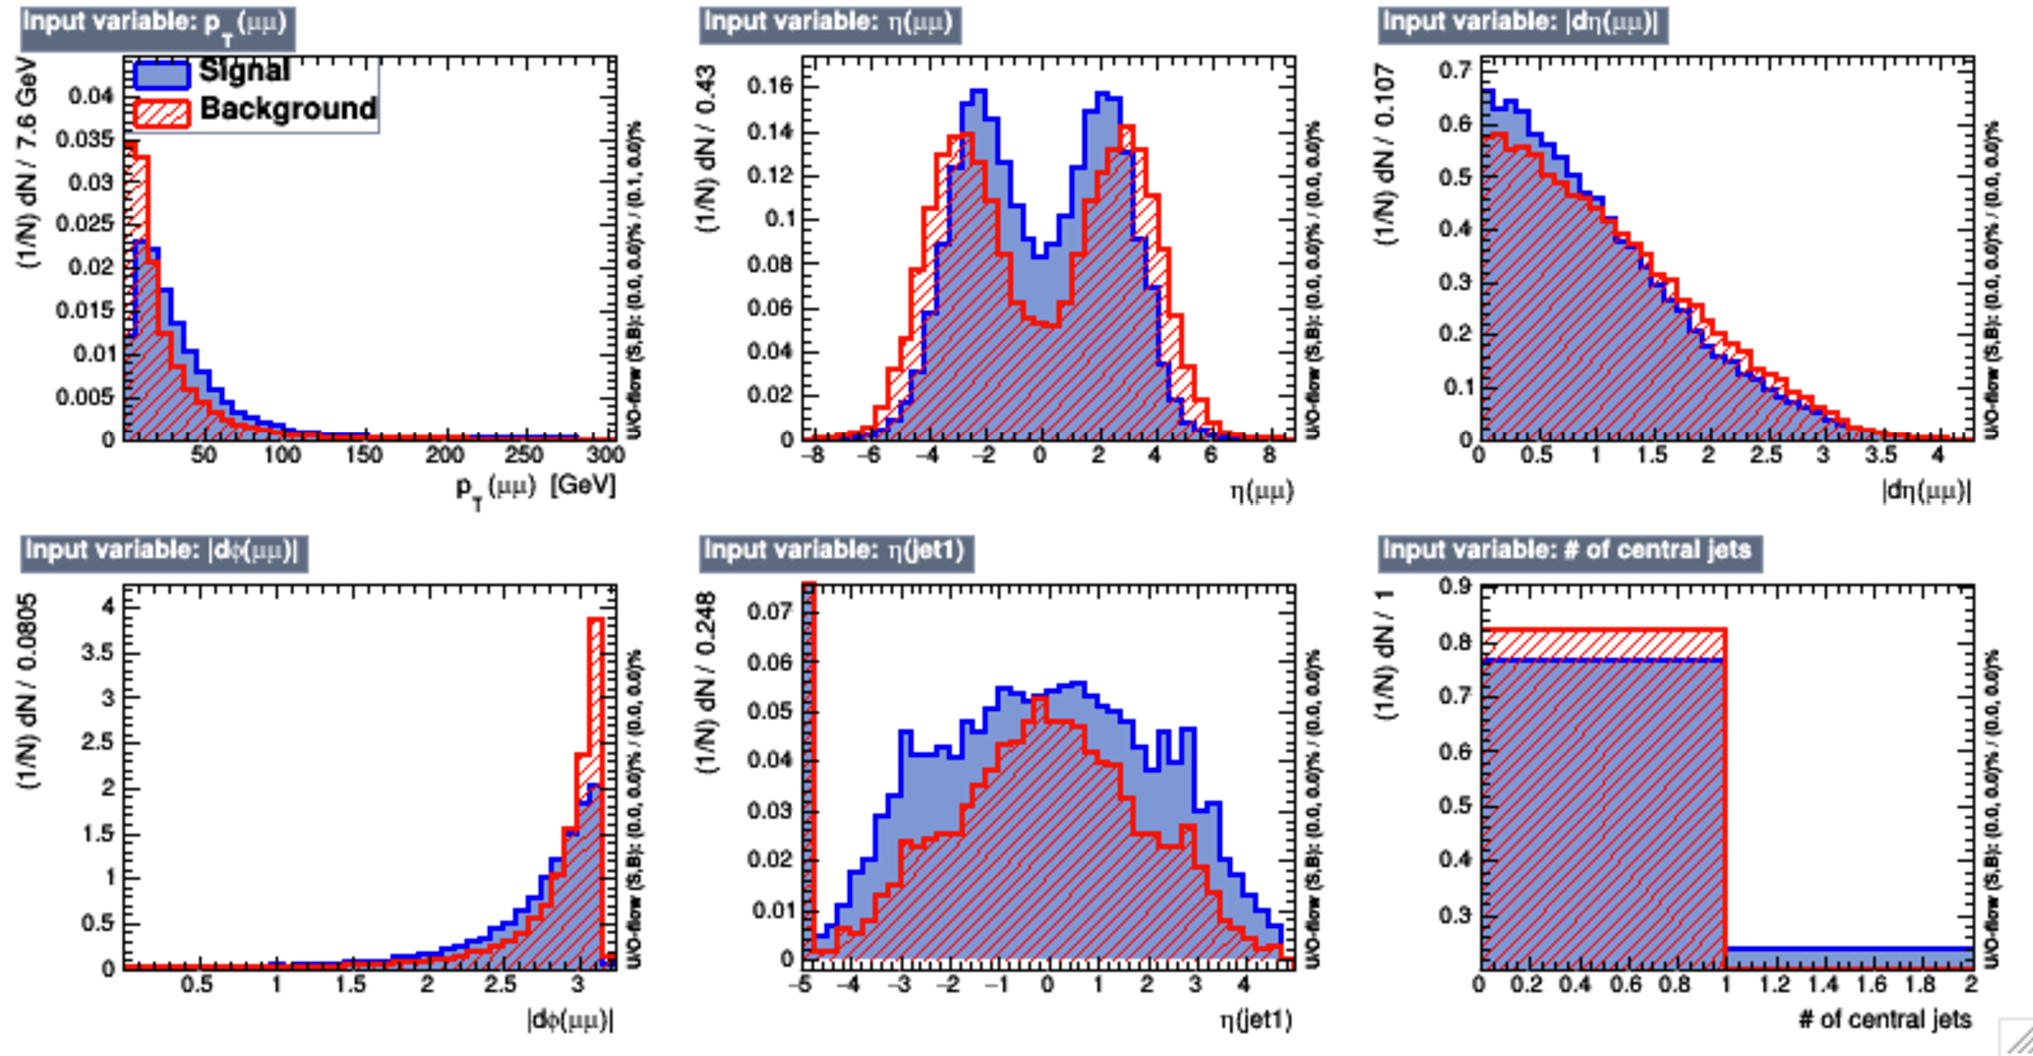
\includegraphics[width=1.0\linewidth]{figures/bdt_training/BDT_in_le1j_all_A.pdf}
%   \includegraphics[width=1.0\linewidth]{figures/bdt_training/BDT_in_le1j_sep_A.pdf}
%   \caption{Some BDT input variables for events with $\le 1$ jets.
%            In the top plots, signal is in blue and background in red.
%            In the bottom plots, the gluon-fusion signal is dark blue, VBF is red, and VH is green,
%            while Drell--Yan and diboson backgrounds are pink, and \ttbar and single top are light blue.}
%   \label{fig:BDT_in_le1j_A}
% \end{figure}

% \begin{figure}
%   \includegraphics[width=1.0\linewidth]{figures/bdt_training/BDT_in_le1j_all_B.pdf}
%   \includegraphics[width=1.0\linewidth]{figures/bdt_training/BDT_in_le1j_sep_B.pdf}
%   \caption{Some BDT input variables for events with $\le 1$ jets.
%            In the top plots, signal is in blue and background in red.
%            In the bottom plots, the gluon-fusion signal is dark blue, VBF is red, and VH is green,
%            while Drell--Yan and diboson backgrounds are pink, and \ttbar and single top are light blue.}
%   \label{fig:BDT_in_le1j_B}
% \end{figure}

% \begin{figure}
%   \includegraphics[width=1.0\linewidth]{figures/bdt_training/BDT_in_eq2j_sep_B.pdf}
%   \caption{Some BDT input variables for events with $= 2$ jets.
%            The gluon-fusion signal is dark blue, VBF is red, and VH is green,
%            while Drell--Yan and diboson backgrounds are pink, and \ttbar and single top are light blue.}
%   \label{fig:BDT_in_eq2j_B}
% \end{figure}

% \begin{figure}
%   \includegraphics[width=1.0\linewidth]{figures/bdt_training/BDT_in_eq2j_all_A.pdf}
%   \includegraphics[width=1.0\linewidth]{figures/bdt_training/BDT_in_eq2j_sep_A.pdf}
%   \caption{Some BDT input variables for events with $= 2$ jets.
%            In the top plots, signal is in blue and background in red.
%            In the bottom plots, the gluon-fusion signal is dark blue, VBF is red, and VH is green,
%            while Drell--Yan and diboson backgrounds are pink, and \ttbar and single top are light blue.}
%   \label{fig:BDT_in_eq2j_A}
% \end{figure}

% \begin{figure}
%   \includegraphics[width=1.0\linewidth]{figures/bdt_training/BDT_in_ge3j_all_A.pdf}
%   \includegraphics[width=1.0\linewidth]{figures/bdt_training/BDT_in_ge3j_sep_A.pdf}
%   \caption{Some BDT input variables for events with $\ge 3$ jets.
%            In the top plots, signal is in blue and background in red.
%            In the bottom plots, the gluon-fusion signal is dark blue, VBF is red, and VH is green,
%            while Drell--Yan and diboson backgrounds are pink, and \ttbar and single top are light blue.}
%   \label{fig:BDT_in_ge3j_A}
% \end{figure}

% \begin{figure}
%   \includegraphics[width=1.0\linewidth]{figures/bdt_training/BDT_in_ge3j_all_B.pdf}
%   \includegraphics[width=1.0\linewidth]{figures/bdt_training/BDT_in_ge3j_sep_B.pdf}
%   \caption{Some BDT input variables for events with $\ge 3$ jets.
%            In the top plots, signal is in blue and background in red.
%            In the bottom plots, the gluon-fusion signal is dark blue, VBF is red, and VH is green,
%            while Drell--Yan and diboson backgrounds are pink, and \ttbar and single top are light blue.}
%   \label{fig:BDT_in_ge3j_B}
% \end{figure}

% \clearpage

% The BDT output distributions for both the inclusive and $\le 1$, $= 2$, and $\ge 3$
% jet trainings can be seen in Figure~\ref{fig:BDT_out}, with the corresponding ROC curves
% in Figure~\ref{fig:BDT_ROC}.  We also performed a multi-classification which assigned
% separate BDT scores for each of the signal and background classes: ggH, VBF, VH, EWK,
% and TOP.  In the end, the binary signal--background classification algorithm, trained
% on the inclusve $\ge 0$ jets sample of events, provided a signal--background separation
% which was as good as any scheme using either the separate-jet trainings or the
% multi-classification algorithm.

% \begin{figure}
%   \includegraphics[width=0.5\linewidth]{figures/bdt_training/BDT_out_ge0j_all.pdf}
%   \includegraphics[width=0.5\linewidth]{figures/bdt_training/BDT_out_le1j_all.pdf}
%   \includegraphics[width=0.5\linewidth]{figures/bdt_training/BDT_out_eq2j_all.pdf}
%   \includegraphics[width=0.5\linewidth]{figures/bdt_training/BDT_out_ge3j_all.pdf}
%   \caption{The BDT output score for events with $\ge 0$ jets (top left), $\leq 1$ jet (top right),
%            $= 2$ jets (bottom left), and $\ge 3$ jets (bottom right).}
%   \label{fig:BDT_out}
% \end{figure}

% \begin{figure}
%   \includegraphics[width=0.5\linewidth]{figures/bdt_training/BDT_ROC_ge0j_all.pdf}
%   \includegraphics[width=0.5\linewidth]{figures/bdt_training/BDT_ROC_le1j_all.pdf}
%   \includegraphics[width=0.5\linewidth]{figures/bdt_training/BDT_ROC_eq2j_all.pdf}
%   \includegraphics[width=0.5\linewidth]{figures/bdt_training/BDT_ROC_ge3j_all.pdf}
%   \caption{The background-rejection vs. signal efficiency ROC curve from the
%            BDT output score for events with $\ge 0$ jets (top left), $\le 1$ jet (top right),
%            $= 2$ jets (bottom left), and $\ge 3$ jets (bottom right).}
%   \label{fig:BDT_ROC}
% \end{figure}

% \clearpage

% \subsection{BDT for Event Categorization}
% \label{bdt_cats}

% In order to optimize the sensitivity of the \Htomm search in a systematic way, the events
% are categorized based on two criteria: the BDT output score and the muon eta information.
% The output score of the BDT is used to separate signal
% from background events, where the score ranges from -1 (background-like) to +1 (signal-like).
% In addition, the maximum $|\eta|$ value of the two candidate muons is used to isolate events with better
% signal-peak resolution. In order to optimize the choice of BDT and $|\eta|$ cuts, we designed and implemented
% a decision tree autocategorizer to create categories by greedily optimizing a metric corresponding
% to the sensitivity which by proxy minimizes the expected upper limit. The BDT training and the autocategorization
% are performed on 50\% of the signal MC events and 100\% of the background MC events.
% After training the autocategorizer on the signal and background MC to determine the categories,
% the expected limits are calculated using data and the remaining 50\% of simulated signal events. Separating the
% signal into separate training and evaluation sets and excluding the data from the training phase ensure an unbiased estimate for the expected limits.

% \begin{figure}[hbp]
%   \centering
%   \includegraphics[width=0.49\linewidth]{figures/bdt_cats/bdt_score_ggH_VBF_DY_ttbar.pdf}
%   \includegraphics[width=0.49\linewidth]{figures/bdt_cats/bdt_score_inclusive_data_mc.png}
%   \caption
%    {The BDT score on the signal and background Monte Carlo (left), where a higher score marks the signal like events.
%     Note \ttbar on the left as the most distinguishable background and VBF on the right as the most distinguishable signal.
%     The BDT score in data is modeled well by the amc@NLO Drell--Yan MC (right). }
%   \label{fig:bdt_score_inclusive}
% \end{figure}

% \subsection{The Auto-Categorizer}

% In order to account for the resolution, the signal and background events are binned in half-GeV bins in the signal
% region of the dimuon mass spectrum, 120 to 130 GeV. The significance in each bin is then given by $S/\sqrt{B}$.
% The significance for independent bins adds in quadrature, so the net significance is given by

% \begin{equation}
% Net~Significance = \sum_{c,i}S_{c,i}^{2}/B_{c,i}
% \end{equation}

% where $i$ labels the bin in the signal region, and $c$ denotes the category. $S_{c,i}$ is the number of expected signal
% events in the $i^{th}$ bin in that category, and $B_{i,c}$ is the number of expected background events in the $i^{th}$ bin.
% By binning finely enough, the central mass bins contribute the most and the resolution is accounted for.

% \begin{figure}[hbp]
%   \centering
%   \includegraphics[width=0.49\linewidth]{figures/bdt_cats/binning_signal_example.png}
%   \includegraphics[width=0.49\linewidth]{figures/bdt_cats/binning_bg_example.png}
%   \caption
%   {An example of the binned signal and background necessary for the significance metric. The binning keeps the most sensitive bins
%    from being drowned out by the others, providing a measure that accounts for both signal--background discrimination and resolution.}
%   \label{fig:binning_example}
% \end{figure}

% On the first iteration, the autocategorizer calculates the net significance for the set of all events, the inclusive set.
% The algorithm then searches over the inclusive set, checking all possible split values of the maximum muon $|\eta|$. Events
% with maximum $|\eta|$ values less than the split go in one candidate category, and those with eta values greater than or equal
% to the split value go into the other candidate category. For every split candidate, the algorithm calculates the net significance
% in the two categories delineated by the split value. The maximum $|\eta|$ cut value that provides the largest gain in significance
% over the inclusive set is stored. The gain is defined in the equation below where $c1$ and $c2$ are the prospective categories
% created from $c$ by splitting on the feature.

% \begin{equation}
% Gain = \sum_{i}S_{c1,i}^{2}/B_{c1,i} + \sum_{i}S_{c2,i}^{2}/B_{c1,i} - \sum_{i}S_{c,i}^{2}/B_{c,i}
% \end{equation}

% The autocategorizer then searches over the BDT score values and stores the BDT score that provides the largest gain in significance.
% The algorithm chooses to split on either the maximum muon $|\eta|$ or the BDT score (whichever has the higher gain), creating two
% categories from the inclusive set of events. At the next iteration, the autocategorizer repeats the procedure for the two new
% categories and chooses to split the category that provides the most gain. This process continues, each time greedily choosing to
% split the category with the most gain, until the number of categories desired is reached.

% %% \begin{figure}[hbp]
% %%   \centering
% %%   \includegraphics[width=0.49\linewidth]{figures/bdt_cats/split_example.png}
% %%   \caption
% %%    {Splitting a category on a feature to form two new categories.}
% %%   \label{fig:split_example}
% %% \end{figure}

% \subsection{Final Categories}

% After training the BDT and autocategorizing based upon the maximum muon $\eta|$ and the BDT score, the resulting categorization is
% simplified by merging a few categories and rounding some of the cuts. Care is taken so that the simplifications do not worsen the
% expected limit. The 13 finalized BDT categories in Figure~\ref{fig:final_categories} show a 23\% improvement compared to using the
% 15 Run~I \Htomm categories. The expected upper limits are evaluated on the same 36~\invfb of 2016 data and signal Monte Carlo in the
% same way for an even comparison. The BDT categories are named such that the numbers go from low sensitivity to high sensitivity, e.g.
% c0 has the lowest expected sensitivity and c12 has the highest expected sensitivity.

% \begin{figure}[hbp]
%   \centering
%   \includegraphics[width=1.0\linewidth]{figures/bdt_cats/final_categories.png}
%   \caption
%    {The final categorization. $|\eta|$ refers to the maximum $|\eta|$ value of the two muons in the dimuon pair. c12 and c9
%     contain the highest proportion of VBF signal events.}
%   \label{fig:final_categories}
% \end{figure}

% %\begin{table}[htb]
% %  \caption{Expected signal and background yields near the signal peak, expected sensitivity from MC, and expected limits from data.}
% %  \label{tab:cat_yields}
% %  \begin{center}
% %    \begin{tabular}{|c|r|r|c|c|c|r|}
% %      \hline\hline
% %      Category  & Signal  & Background & $\mathrm{S / B}$ (\%) & $\mathrm{S / \sqrt{B}}$ & Sensitivity & Limit \\  %% & Signal events
% %      \hline\hline
% %      c0        &  13.47  & 13660.7    & 0.098                 & 0.115                   & 0.124       & 19.30 \\  %% &  19.21
% %      c1        &   3.74  &   982.5    & 0.381                 & 0.119                   & 0.130       & 19.80 \\  %% &   5.48
% %      c2        &  14.97  &  7961.8    & 0.188                 & 0.167                   & 0.179       & 15.30 \\  %% &  21.97
% %      c3        &   4.15  &   807.8    & 0.513                 & 0.146                   & 0.173       & 14.80 \\  %% &   5.95
% %      c4        &   9.89  &  1516.0    & 0.652                 & 0.254                   & 0.271       &  8.47 \\  %% &  13.79
% %      c5        &   9.46  &  1145.7    & 0.826                 & 0.279                   & 0.302       &  7.66 \\  %% &  12.56
% %      c6        &  14.19  &  2270.6    & 0.625                 & 0.297                   & 0.323       &  7.28 \\  %% &  20.44
% %      c7        &  27.40  &  6907.3    & 0.396                 & 0.329                   & 0.356       &  6.72 \\  %% &  40.39
% %      c8        &  37.88  & 11766.1    & 0.322                 & 0.349                   & 0.374       &  6.25 \\  %% &  52.26
% %      c9        &   6.22  &   400.2    & 1.555                 & 0.311                   & 0.345       &  7.59 \\  %% &   8.97
% %      c10       &  14.05  &  1575.3    & 0.891                 & 0.354                   & 0.380       &  6.53 \\  %% &  20.75
% %      c11       &  10.25  &   812.2    & 1.262                 & 0.359                   & 0.388       &  6.34 \\  %% &  13.91
% %      c12       &   9.67  &   407.6    & 2.373                 & 0.479                   & 0.550       &  4.67 \\  %% &  14.33
% %      %% \hline
% %      %% Inclusive & 170.16  & 45540.3    & 0.373                 & 0.797                   & 0.858       &  1.85 \\  %% & 250.07
% %      \hline\hline
% %    \end{tabular}
% %  \end{center}
% %\end{table}

% \begin{table}[htb]
%   \caption{Full Width Half Max (FWHM) of the signal peak, expected signal and background yields within the FWHM,
%            expected sensitivity from MC, and expected limits from data.}
%   \label{tab:cat_yields}
%   \begin{center}
%     \begin{tabular}{|c|r|r|c|c|c|r|r|}
%       \hline\hline
%       Category  & Signal FWHM (GeV) & Signal & Background & $\mathrm{S / B}$ (\%) & $\mathrm{S / \sqrt{B}}$ & Sensitivity & Limit \\  %% & Signal events
%       \hline\hline
%       c0          &        4.4           &      13.4826         &    14187.6        &     0.000950307    &     0.113193        & 0.124       & 19.30 \\
%       c1          &        5.8           &      3.52888         &    970.875        &     0.00363474     &     0.113255        & 0.130       & 19.80 \\
%       c2          &        5.8           &      14.2112         &    8248.64        &     0.00172286     &     0.156473        & 0.179       & 15.30 \\
%       c3          &        6.0           &      3.82012         &    779.594        &     0.00490015     &     0.136818        & 0.173       & 14.80 \\
%       c4          &        3.0           &      9.92363         &    1609.08        &     0.00616729     &     0.24739         & 0.271       &  8.47 \\
%       c5          &        2.8           &      8.5825          &    1028.08        &     0.00834811     &     0.267671        & 0.302       &  7.66 \\
%       c6          &        4.0           &      14.1224         &    2371.09        &     0.00595611     &     0.290025        & 0.323       &  7.28 \\
%       c7          &        4.2           &      26.3575         &    6904.16        &     0.00381762     &     0.317211        & 0.356       &  6.72 \\
%       c8          &        3.6           &      35.6493         &    11187.4        &     0.00318655     &     0.337043        & 0.374       &  6.25 \\
%       c9          &        4.0           &      6.12457         &    451.281        &     0.0135715      &     0.288305        & 0.345       &  7.59 \\
%       c10         &        4.0           &      13.9349         &    1667.59        &     0.00835632     &     0.34124         & 0.380       &  6.53 \\
%       c11         &        3.0           &      9.59255         &    765.226        &     0.0125356      &     0.346768        & 0.388       &  6.34 \\
%       c12         &        4.0           &      9.58541         &    420.983        &     0.0227691      &     0.467173        & 0.550       &  4.67 \\
%       \hline\hline
%     \end{tabular}
%   \end{center}
% \end{table}


% \subsection{Validating The Categories}

% It is important that the signal is correctly modeled in each category in order to report an accurate expected upper limit.
% %% Insofar, the Monte Carlo is compared to the Data in the sidebands.
% Figure~\ref{fig:valid_bdt_incl} shows the data-to-MC agreement for the BDT features
% for the inclusive set of events with dimuon mass greater than 60~GeV.

% \begin{figure}[hbp]
%   \centering
%   \includegraphics[width=0.32\linewidth]{figures/bdt_cats/dimu_eta_root.png}
%   \includegraphics[width=0.32\linewidth]{figures/bdt_cats/dimu_abs_dEta_root.png}
%   \includegraphics[width=0.32\linewidth]{figures/bdt_cats/dimu_abs_dPhi_root.png}
%   \includegraphics[width=0.32\linewidth]{figures/bdt_cats/nJetsCent_root.png}
%   \includegraphics[width=0.32\linewidth]{figures/bdt_cats/dijet1_mass_root.png}
%   \includegraphics[width=0.32\linewidth]{figures/bdt_cats/dijet1_abs_dEta_root.png}
%   \includegraphics[width=0.32\linewidth]{figures/bdt_cats/nJetsFwd_root.png}
%   \includegraphics[width=0.32\linewidth]{figures/bdt_cats/dijet2_mass_root.png}
%   \includegraphics[width=0.32\linewidth]{figures/bdt_cats/dijet2_abs_dEta_root.png}
%   \caption
%    {Validation of BDT input variables in inclusive events.}
%   \label{fig:valid_bdt_incl}
% \end{figure}

% The Data and Monte Carlo agree very well especially in the dimuon mass distribution, where the agreement is within 5\%.
% Furthermore, Fig.~\ref{fig:valid_bdt_c12a} and~\ref{fig:valid_bdt_c12b} show the Data/MC agreement for c12,
% the most sensitive, most VBF-like category. The BDT distribution in quantile is presented in Fig.~\ref{fig:bdt_quantile}
% with the systematic uncertainties given by the JES and PU.

% \begin{figure}[hbp]
%   \centering
%   \includegraphics[width=0.32\linewidth]{figures/bdt_cats/dimu_eta_c12.png}
%   \includegraphics[width=0.32\linewidth]{figures/bdt_cats/dimu_abs_dEta_c12.png}
%   \includegraphics[width=0.32\linewidth]{figures/bdt_cats/dimu_abs_dPhi_c12.png}
%   \includegraphics[width=0.32\linewidth]{figures/bdt_cats/nJetsCent_c12.png}
%   \includegraphics[width=0.32\linewidth]{figures/bdt_cats/dijet1_mass_c12.png}
%   \includegraphics[width=0.32\linewidth]{figures/bdt_cats/dijet1_abs_dEta_c12.png}
%   \includegraphics[width=0.32\linewidth]{figures/bdt_cats/nJetsFwd_c12.png}
%   \includegraphics[width=0.32\linewidth]{figures/bdt_cats/dijet2_mass_c12.png}
%   \includegraphics[width=0.32\linewidth]{figures/bdt_cats/dijet2_abs_dEta_c12.png}
%   \caption
%    {Data/MC agreement for the most sensitive category.}
%   \label{fig:valid_bdt_c12a}
% \end{figure}

% \begin{figure}[hbp]
%   \centering
%   \includegraphics[width=0.32\linewidth]{figures/bdt_cats/dimu_mass_Roch_c12.png}
%   \includegraphics[width=0.32\linewidth]{figures/bdt_cats/dimu_pt_c12.png}
%   \includegraphics[width=0.32\linewidth]{figures/bdt_cats/MET_c12.png}
%   \includegraphics[width=0.32\linewidth]{figures/bdt_cats/nBMed_c12.png}
%   \includegraphics[width=0.32\linewidth]{figures/bdt_cats/jet1_eta_c12.png}
%   \includegraphics[width=0.32\linewidth]{figures/bdt_cats/jet2_eta_c12.png}
%   \caption
%    {Data/MC agreement for the most sensitive category.}
%   \label{fig:valid_bdt_c12b}
% \end{figure}

% \begin{figure}[hbp]
% \centering
% \includegraphics[width=0.7\linewidth]{figures/bdt_cats/BdtOnH_QM_bkg.png}
%   \caption{The BDT distribution in quantile in data and MC. The systematic uncertainty is given by the JES and PU.}
%   \label{fig:bdt_quantile}
% \end{figure}

% Again, the Data and Monte Carlo agree very well. Lastly, it is important that the BDT score is mass independent. One way to
% show this is to demonstrate that the classifier score remains the same for signal Monte Carlo with different values of
% $M_{Higgs}$. If the BDT score does not change as the mass changes, then it is clearly mass independent. As shown in
% Figure~\ref{fig:mass_independence}, the BDT score does not change significantly with the dimuon mass.

% \begin{figure}[hbp]
%   \centering
%   \includegraphics[width=0.49\linewidth]{figures/bdt_cats/BDT_Score_GGF_M125_vs_M120.png}
%   \includegraphics[width=0.49\linewidth]{figures/bdt_cats/BDT_Score_GGF_M125_vs_M130.png}
%   \includegraphics[width=0.49\linewidth]{figures/bdt_cats/BDT_Score_VBF_M125_vs_M120.png}
%   \includegraphics[width=0.49\linewidth]{figures/bdt_cats/BDT_Score_VBF_M125_vs_M130.png}
%   \caption
%    {Plots showing the agreement between $M_{Higgs}$ = 125 GeV vs. 120 GeV and $M_{Higgs}$ = 125 GeV vs. 130 GeV for ggH and VBF.}
%   \label{fig:mass_independence}
% \end{figure}
